\documentclass[make,article,submit,pdftex]{Definitions/mdpi}

\usepackage{amsthm}
\usepackage{booktabs}
\usepackage{multirow}
\usepackage{float}
\usepackage{enumitem}
\providecommand{\KL}{}\renewcommand{\KL}{\mathrm{KL}}
\providecommand{\E}{}\renewcommand{\E}{\mathbb{E}}
\newcommand{\risk}{\mathrm{risk}}
\newcommand{\haz}{\mathrm{haz}}
\newtheorem{prop}{Proposition}
\setlength{\emergencystretch}{3em}
% macros that some versions of the MDPI class do not define (no-ops where undefined)
\providecommand{\hreflink}[1]{}
\providecommand{\acknowledgments}[1]{\paragraph{Acknowledgments.} #1}
\providecommand{\TitleCitation}[1]{}
\providecommand{\AuthorCitation}[1]{}

%% Front matter -- fill in the author block before submission.
\firstpage{1}
\makeatletter
\setcounter{page}{\@firstpage}
\makeatother
\pubvolume{1}
\issuenum{1}
\articlenumber{0}
\pubyear{2026}
\copyrightyear{2026}
\datereceived{}
\daterevised{}
\dateaccepted{}
\datepublished{}
\hreflink{}

\Title{Why Fixed Per-Step Risk Budgets Waste KL When Preventing Repetition Loops}
\TitleCitation{Why Fixed Per-Step Risk Budgets Waste KL When Preventing Repetition Loops}
\Author{[Author Name] $^{1}$}
\AuthorNames{[Author Name]}
\AuthorCitation{[Author Surname], [I.]}
\address{%
$^{1}$ \quad [Affiliation, city, country]}
\corres{Correspondence: [email address]}

\abstract{Repetition-suppressing decoders usually fix a risk budget at every step, whereas what matters is the probability that a loop occurs anywhere in the sequence. We ask why a fixed per-step budget can waste KL divergence from the model, and by how much. We show that the loop probability falls by the visit-weighted sum of per-step hazard reductions, that to second order the cheapest allocation holds the price of risk (the Lagrange multiplier) constant, and that a fixed budget implies widely varying prices, its excess cost being one plus their squared coefficient of variation. In exactly solved finite-state systems a fixed price stays within 12.5\% of the minimum KL, whereas a fixed budget costs 1.3 to about 700 times the minimum, with and without infeasible budgets; the ratio tends to a finite limit (707 in the base system) as the reduction goes to zero. On a character-level language model a fixed price reached zero observed loops at 39 bits per generation, while every fixed budget below 1 tested cost at least 458 bits. These are observed counts at one temperature, not guarantees; KL measures distortion, not text quality; and about 98\% of each decoder's path KL lies beyond the cost of moving the loop probability.}

\keyword{repetition loops; decoding; KL divergence; Lagrange multiplier; constrained decoding; language models}

\begin{document}
\section{Introduction}\label{sec:intro}

Autoregressive language models sometimes fall into repetition loops: the model emits a short span and then reproduces it until the sample is dominated by a fixed cycle. Most remedies are decoding rules applied one token at a time. They look at the next-token distribution and at a short history, and they penalize or forbid candidates that would repeat recent text. A common design fixes how much repetition risk a single step may carry, a \emph{per-step risk budget}, and re-solves it at every step. Whether a loop occurs, however, is a property of the whole sequence. The distortion that a rule introduces, measured here as the KL divergence of the controlled generation from the model's own, is spent at every step whether or not a loop is at stake.

We ask one question: \emph{why can a fixed per-step risk budget waste KL divergence when the goal is to prevent a loop anywhere in the generated sequence, and by how much?} The answer we give is not that token-by-token control is inefficient in itself. A one-step controller has two dual parameters, a risk budget and its Lagrange multiplier, the \emph{price} of risk. Holding the budget fixed and holding the price fixed are different designs. We show that the cheapest way to lower the probability of a loop holds the price constant across histories, and that a fixed budget instead induces prices that vary by orders of magnitude, which is where the KL is wasted.

\subsection{Contributions}
\begin{enumerate}[leftmargin=*,itemsep=2pt]
\item \textbf{A mechanism with an explicit waste law (Section~\ref{sec:theory}).} The probability of a loop falls by the expected sum of per-step hazard reductions, and the minimum KL for a given reduction is known in closed form. To second order, a controller that reduces the hazard by $\Delta(h)$ at history $h$ costs a factor $1+\mathrm{CV}^2$ more than the optimum, where $\mathrm{CV}$ is the coefficient of variation of its implied per-step prices; a fixed budget costs at least the reciprocal of the share of the event's variance on the histories it touches. These are elementary consequences of known tools, which we credit in Section~\ref{sec:related}; what we add is their use as an accounting of repetition control.
\item \textbf{An exact test, with infeasibility separated from allocation (Section~\ref{sec:small}).} In finite-state systems where the optimum, the controllers and the loop probabilities are computed exactly, a fixed price stays within 12.5\% of the minimum KL in every setting, whereas a fixed budget costs between 1.3 times the minimum and, for the smallest reductions, about 700 times (where both costs are below $10^{-10}$ bits). The excess is present with no infeasible budget at all, and removing infeasibility does not remove it.
\item \textbf{A qualified, descriptive test on a language model (Section~\ref{sec:real}).} On a character-level model with a validated loop detector we compare a fixed-price rule with a fixed-budget rule at similar observed loop counts, report the per-step prices the budget rule realizes, and state which findings of the exact systems the language-model data support and which remain hypotheses.
\end{enumerate}

\subsection{Scope}
Recurrence-risk decoding is used here as an instrument for studying the question, not proposed as a practical decoder. Observed loop counts are counts at one temperature on a few models, not guarantees. KL divergence is a measure of distortion, not of readability or text quality. The language-model estimates are descriptive; they do not say how much distortion a practical decoder could save. Models beyond the primary one, the loop-detector validation, baseline details, a pilot human evaluation, a rollout-based hazard estimate and the implementation defects found along the way are in the appendices.

\section{Related Work}\label{sec:related}

\textbf{Mathematical tools.} The one-step problem of Section~\ref{sec:setup} is an I-projection of a distribution onto a linear family, whose solution is an exponential tilt of the reference \cite{csiszar1975idivergence}; its Lagrange dual is a convex program \cite{boyd2004convex}. The chain rule for relative entropy used in Section~\ref{sec:theory} is standard \cite{cover2006elements}. The optimal event-level policy is a Doob $h$-transform of the reference process \cite{doob1957conditional}, and the sequential form of KL-regularized control, in which the optimal controlled transition reweights the uncontrolled one by an exponentiated value function, is the theory of linearly solvable control \cite{kappen2005linear,todorov2007linearly}. The change in the probability of an event under a changed policy as an expected sum of per-step advantages is the performance-difference identity of reinforcement learning \cite{kakade2002approximately}. Equalizing the marginal cost of distortion across components is the equal-slope condition of constrained allocation \cite{cover2006elements,boyd2004convex}; in constrained Markov decision processes a cumulative constraint is handled by a single Lagrange multiplier, whereas a constraint imposed at every step is a different and more restrictive class \cite{altman1999constrained,achiam2017constrained}. We do not claim any of these identities as new.

\textbf{Local token control and global distortion.} That constraining or reweighting a language model token by token induces a sequence distribution different from a sequence-level target is established outside the repetition-loop setting. Controlled decoding \cite{mudgal2024controlled} learns a value function to steer per-token choices toward a KL-regularized reward optimum; twisted Sequential Monte Carlo \cite{zhao2024twisted} and its extension to syntactic and semantic constraints \cite{loula2025syntactic} correct a token-level proposal by particle reweighting because the proposal alone does not sample from the target; adaptive weighted rejection sampling \cite{lipkin2025awrs} makes constrained token-level sampling exact for a broad class of constraints. We do not claim that a gap between local and global control is new. The contribution is narrower: for repetition loops, the gap is a statement about holding a budget fixed rather than a price, it has a closed-form size to second order, and it can be computed exactly in a small system and checked on a language model.

\textbf{Decoding strategies for repetition.} Temperature sampling rescales logits by $1/T$. Nucleus sampling \cite{holtzman2020curious} truncates to the smallest set of tokens with cumulative probability above $p$. Repetition penalty \cite{keskar2019ctrl} divides the logit of every previously generated token by a constant. Typical sampling \cite{meister2023typical} and Mirostat \cite{basu2021mirostat} control the surprisal of the sampled token. No-repeat $n$-gram blocking \cite{paulus2018deep} zeroes the probability of any token that would complete an already-seen $n$-gram. History-aware baselines used here are a longest-suffix-match heuristic (SuffixMatch, our own and not attributed to any publication), an FSD-style decoder adapted from Frustratingly Simple Decoding \cite{yang2023frustratingly}, and a decoder that applies the penalty of the LZ Penalty \cite{ginart2025lzpenalty} with adapted history handling; their relation to the published methods is stated in Appendix~\ref{app:baselines}. Loop onset is treated as a survival time, estimated with Kaplan--Meier \cite{kaplan1958nonparametric}; the character-level models are decoder-only Transformers \cite{vaswani2017attention}.

\section{Setting and Definitions}\label{sec:setup}

Let $p(\cdot\mid h)$ be the reference next-token distribution given a history $h$, the model at sampling temperature $T$ ($p=\mathrm{softmax}(\mathrm{logits}/T)$). A decoder samples from a kernel $q(\cdot\mid h)$. Over generations of $N$ tokens these define path measures $P$ (the reference) and $Q$ (the decoder). \textbf{Every KL divergence in this paper is in bits.} By the chain rule $\KL(Q\Vert P)=\E_Q\sum_t \KL(q_t\Vert p_t)$, so the path KL of a decoder is estimated by summing the per-step divergences along its own samples; a ``per-step mean'' divides that sum by the fixed generation length $N$.

\textbf{The loop event.} A detector $\mathcal{L}$ defines the loop onset $\tau=\min\{t\le N:\mathcal{L}(x_{1:t})=1\}$ ($\tau=\infty$ if no such $t$ exists), and the event of interest is $E=\{\tau\le N\}$, a loop by the end of the generation. Appendix~\ref{sec:event} develops the detector used on the character-level model and states its limitations. For a history $h$ that has not yet looped and a candidate token $v$, the \emph{event-to-go hazard} is
\begin{gather*}
H(h,v)=P(E\mid h,v),\qquad H(h,v)=1\ \text{if $v$ completes a loop at once},\\
V(h)=\textstyle\sum_v p(v\mid h)H(h,v)=P(E\mid h).
\end{gather*}
In a finite-state system $H$ is computed exactly (Section~\ref{sec:small}); on a language model it can only be estimated (Appendix~\ref{sec:hazard-transfer}).

\textbf{One-step controllers.} Every controller considered is a one-step KL projection of $p(\cdot\mid h)$ for a risk signal $r(h,v)\ge 0$:
\begin{equation}\label{eq:projection}
\min_q \KL(q\Vert p)\ \ \text{s.t.}\ \ \E_q[r]\le b,\qquad\text{with solution}\qquad q_\lambda(v)\propto p(v)\,e^{-\lambda r(v)} .
\end{equation}
The budget $b$ and the multiplier $\lambda\ge 0$ are dual to one another: for a given history, each determines the other, and $\lambda$ is the \emph{price} of risk, the marginal KL paid per unit of risk removed. If $\E_p[r]\le b$ the constraint is inactive ($\lambda=0$, $q=p$); if $b<\min_v r(v)$ it is infeasible. \textbf{Rule for an unmet budget:} when $b\le\min_vr(v)$ (up to a numerical tolerance) the controller samples from $p$ restricted to the minimum-risk actions $\{v:r(v)=\min r\}$ and renormalized, which is the $\lambda\to\infty$ limit of \eqref{eq:projection} and the minimum-KL distribution among those attaining the smallest achievable risk; the step is recorded as infeasible when $b<\min_vr(v)$. The same rule is used in every exact experiment and in the language-model decoder (Appendix~\ref{app:baselines}). What differs between decoders is which of the two is held fixed over the generation:
\begin{itemize}[leftmargin=*,itemsep=1pt]
\item \textbf{fixed budget (FB):} the same $b$ at every step and history; the price $\lambda(h)$ is whatever satisfies $\E_q[r]=b$;
\item \textbf{fixed price (FP):} the same $\lambda$ at every step and history; the budget $b(h)=\E_{q_\lambda}[r]$ then adapts to the history.
\end{itemize}
The recurrence-risk decoder studied below uses the recurrence risk
\[
r(v)=\frac1{N_o}\sum_{n=n_{\min}}^{n_{\max}}\mathbf{1}\big[(\text{last }n{-}1\text{ tokens},v)\text{ has occurred earlier}\big],\qquad N_o=n_{\max}-n_{\min}+1;
\]
its \textsc{dual} mode is FB (it solves \eqref{eq:projection} exactly at every step), its \textsc{fixed} mode is FP, and its \textsc{adaptive} mode sets $\lambda$ by a heuristic with no guarantee. Appendix~\ref{app:baselines} gives the solver and its numerical tolerances. In the exact system of Section~\ref{sec:small} the risk signal is the exact hazard, $r=H$.

The \textbf{event-level optimum} $Q^\star$ minimizes $\KL(Q\Vert P)$ subject to $Q(E)=\epsilon$. It is a benchmark defined on whole sequences, and Section~\ref{sec:theory} shows that it is realized by a causal sequential rule that uses the hazard with one multiplier for the whole generation.

\section{Theory}\label{sec:theory}

\subsection{The cost of changing a loop probability}\label{ssec:bernoulli-bound}
Let $Q$ and $P$ be path measures on a common sequence space and $E$ any event. The chain rule for relative entropy applied to $Z=\mathbf{1}[E]$ gives
\begin{multline}\label{eq:decomp}
\KL(Q\Vert P)=d_{\mathrm{Ber}}\big(Q(E)\Vert P(E)\big)+Q(E)\,\KL\big(Q(\cdot\mid E)\Vert P(\cdot\mid E)\big)\\
+\big(1-Q(E)\big)\,\KL\big(Q(\cdot\mid E^c)\Vert P(\cdot\mid E^c)\big),
\end{multline}
with $d_{\mathrm{Ber}}(a\Vert b)=a\log_2\frac ab+(1-a)\log_2\frac{1-a}{1-b}$. It needs no Markov structure and no assumption about decoding. The last two terms are non-negative and vanish for $Q(\cdot\mid E)=P(\cdot\mid E)$ and $Q(\cdot\mid E^c)=P(\cdot\mid E^c)$, which is compatible with every value of $Q(E)$. They are the distortion of the conditional shape of the generation on each side of the event, the part of a divergence that is not needed to move the event probability.

\begin{prop}[Minimum KL to move an event probability]\label{prop:min}
With $p=P(E)\in(0,1)$, $\min_{Q:\,Q(E)=\epsilon}\KL(Q\Vert P)=d_{\mathrm{Ber}}(\epsilon\Vert p)$, attained uniquely by $Q^\star(x)=P(x)\,\epsilon/p$ for $x\in E$ and $Q^\star(x)=P(x)(1-\epsilon)/(1-p)$ for $x\notin E$.
\end{prop}

\begin{prop}[A causal realization of the optimum]\label{prop:causal}
Let $2^{-\lambda}=\epsilon(1-p)/[p(1-\epsilon)]$, so that $Q^\star(x)\propto P(x)\,2^{-\lambda\mathbf{1}[x\in E]}$. For a history $h$ that has not triggered $E$,
\[
Q^\star(v\mid h)\ \propto\ P(v\mid h)\,\big[1-(1-2^{-\lambda})\,H(h,v)\big],
\]
a causal sequential rule that uses the exact hazard with one multiplier $\lambda$ for the whole generation.
\end{prop}

Both propositions are standard (Section~\ref{sec:related}); proofs are in Appendix~\ref{app:proofs}. They fix the benchmark: the minimum distortion for a loop probability $\epsilon$ is $d_{\mathrm{Ber}}(\epsilon\Vert p)$, a causal rule attains it when the exact hazard is available, so the gap measured below is not a statement about causality. Resampling a generation until $E$ does not occur realizes $Q=P(\cdot\mid E^c)$ at $\epsilon=0$, with $\KL=-\log_2(1-p)=d_{\mathrm{Ber}}(0\Vert p)$ bits and $1/(1-p)$ expected generations; it attains the bound but is not a streaming decoder.

\subsection{Where the loop probability goes: an exact accounting}\label{ssec:accounting}
For a Markov controller with kernels $q$, write $\Delta(h)=\E_{p}[H(h,\cdot)]-\E_{q}[H(h,\cdot)]$ for the one-step hazard reduction at history $h$, $\sigma^2(h)=\mathrm{Var}_{p(\cdot\mid h)}[H(h,\cdot)]$, and $w_Q(h)$, $w_P(h)$ for the probabilities that $Q$ and $P$ visit $h$ without having looped.

\begin{prop}[Exact accounting]\label{prop:accounting}
(a) $P(E)-Q(E)=\sum_h w_Q(h)\,\Delta(h)$. (b) $\sum_h w_P(h)\,\sigma^2(h)=p(1-p)$.
\end{prop}
Part (a) is the performance-difference identity \cite{kakade2002approximately} for the event; it says that the one-step hazard reduction is the right currency: the loop probability drops by exactly the visit-weighted sum of per-step reductions of the expected hazard. Part (b) is the law of total variance for the martingale $V(h_t)$ under $P$: the variance $p(1-p)$ of the event indicator is spread over histories as $w_P\sigma^2$, and a history with $\sigma^2(h)=0$ cannot change the loop probability at any price.

\subsection{Budget versus price: a second-order waste law}\label{ssec:wastelaw}
For small relative reductions the one-step cost is quadratic, $\KL(q\Vert p)\approx \Delta^2/(2\sigma^2\ln 2)$ bits, and the price implied by a reduction $\Delta$ is $\lambda_h=\Delta(h)/\sigma^2(h)$ (in nats per unit of hazard). Define
\[
D=\sum_h w_P\Delta,\qquad K_2=\frac1{2\ln2}\sum_h w_P\frac{\Delta^2}{\sigma^2},\qquad \pi_h=\frac{w_P\sigma^2}{p(1-p)},
\]
and let $\mathrm{CV}^2=\mathrm{Var}_\pi(\lambda_h)/\E_\pi[\lambda_h]^2$ be the squared coefficient of variation of the implied prices under the distribution $\pi$ over histories, and $\varphi=\sum_{h:\,\Delta(h)>0}\pi_h$ the share of the event's variance on the histories the controller touches.

\begin{prop}[Waste law]\label{prop:waste}
(i) Among all allocations with total reduction $D$, $K_2$ is minimal exactly when $\lambda_h$ is constant, and then $K^\star=D^2/(2\ln 2\,p(1-p))$, the second-order expansion of $d_{\mathrm{Ber}}(p-D\Vert p)$.
(ii) For any allocation, $K_2/K^\star=1+\mathrm{CV}^2\ \ge\ 1/\varphi$.
(iii) $\KL=K_2\,(1+o(1))$ when $\max_h\Delta/\sigma\to0$.
\end{prop}
The first part says that, to second order, the cheapest allocation holds the price constant, which is the fixed-price rule. The second part is algebra on $K_2$: the excess cost is the dispersion of the prices an allocation implies, and it is at least the reciprocal of the share of the event's variance on the histories that receive any reduction (Cauchy--Schwarz on the touched histories). Both statements concern the second-order cost $K_2$. The exact KL satisfies them only in the second-order regime: it agrees with $K_2$ as $D\to0$ (part (iii)), and away from it the exact ratio can be smaller than $1+\mathrm{CV}^2$ or $1/\varphi$ (Section~\ref{ssec:lawtest}).

\textbf{What a fixed budget does.} Under a fixed budget $b$ the reduction at a history is $\Delta(h)=(V(h)-b)_+$, where $V(h)$ is the hazard level. The controller acts only where the level exceeds $b$ and ignores how much variance, hence how cheap leverage, a history holds. Two consequences follow. First, as the target reduction $D$ shrinks, $b$ rises toward the largest hazard level $V_{\max}$ and the touched histories shrink to those at that level; the second-order waste then settles at the finite value $1/\varphi_{\max}$, the reciprocal of the share of $p(1-p)$ held by the histories at $V_{\max}$. It does not grow without limit, but it can be large when the maximal-level histories are rare and carry little variance, and both costs go to zero with $D$ (the ratio can be large while the absolute difference is negligible). Second, histories with small $\sigma^2$ and $V>b$ receive a reduction at a very high implied price; at the extreme the budget is below the floor $\min_vH(h,v)$ and the step is infeasible, which is an infinite price. A fixed price has $\mathrm{CV}=0$ to second order by construction.

\textbf{Outside the second-order regime} the exact optimum is the affine rule of Proposition~\ref{prop:causal}, an exponential tilt of a transformed hazard with one multiplier, and a fixed-price exponential tilt of the hazard itself is not exactly optimal; Section~\ref{sec:small} measures how close it is. Proposition~\ref{prop:waste} is a statement about the hazard as risk signal. A different risk signal, such as the recurrence risk on a language model, changes $\sigma^2$ and $\Delta$ but not the allocation principle; whether the quantitative law carries over is a question for the experiments, not for the proposition.

\section{An Exact Test in Small Systems}\label{sec:small}

\subsection{Construction}
A 20-state Markov chain has a diffuse ``safe'' region from which a small probability (0.05) leads to a gateway state. The gateway is not itself a repeat, but it moves with probability 0.75 into a tight two-cycle (0.80 self-reinforcing in either direction); the transition matrix is tempered at 0.6. The chain starts in state 0. A step \emph{repeats} if the entered state is already in the trailing window of the last $W=2$ states, and a \emph{loop} is $R$ consecutive repeats within the horizon of $N$ transitions: $R=1$ is the first entry of a repeated state, and larger $R$ is a persistent cycle, closer to the detector used on text, which requires a span to repeat five times. The base system has $R=1$, $N=6$ and a reference loop probability $p=0.690024$ computed exactly. The hazard $H$ is computed by exact backward dynamic programming over (state, window, run length, steps remaining); a loop is absorbing, and a trajectory that loops pays the KL of the decisions up to and including the one that caused it. Every ``KL'' below is an exact expected path divergence in bits, and every loop probability is exact; nothing is simulated. One-step problems are solved by a single routine with an expanding bracket for the multiplier (doubling from $\lambda=1$ until the budget is met, up to $10^9$) followed by bisection; the final distribution is checked against the budget, and a solve that fails its check raises an error and is never counted as a success. To test robustness we repeat everything for eight systems that vary the gateway probability, the strength of the funnel, the temperature, the horizon and $R\in\{1,2,3\}$ (Table~\ref{tab:robust}).

\subsection{Controllers}
All controllers use the exact hazard as risk signal, $r=H$, and are calibrated by bisection on a single scalar so that their exact loop probability equals the target $\epsilon$. They form a ladder in which each rung changes one thing:
\begin{itemize}[leftmargin=*,itemsep=1pt]
\item \textbf{fixed budget} $\E_q[H]\le b$ at every step (the controller of Section~\ref{sec:setup}). If the budget is below the floor $\min_vH$ the step is infeasible, and the controller samples from $p$ restricted to the minimum-risk actions (the rule of Section~\ref{sec:setup}, identical in the language-model decoder);
\item \textbf{always-feasible budget} $\E_q[H]\le \min_v H+\rho\,(\E_p[H]-\min_v H)$, one scalar $\rho$ for the whole generation, which cannot be infeasible;
\item \textbf{best budget schedule}: step-dependent budgets $b_1,\dots,b_N$ independent of the history, optimized numerically;
\item \textbf{fixed price} $q\propto p\,2^{-\lambda H}$ with one $\lambda$ (an exponential tilt);
\item the \textbf{optimum}: the affine rule of Proposition~\ref{prop:causal}, whose KL is $d_{\mathrm{Ber}}(\epsilon\Vert p)$. We verify that its sequential computation agrees with this closed form to $<10^{-9}$ at every target and that Proposition~\ref{prop:accounting} holds to $<10^{-9}$ in every run.
\end{itemize}

\subsection{Results: the ladder}\label{ssec:ladder}
\begin{table}[H]
\centering
\caption{Base system ($R{=}1$, $N{=}6$, reference loop probability $p=0.6900$): total path KL in bits and as a multiple of the minimum $d_{\mathrm{Ber}}(\epsilon\Vert p)$, for each rule of the ladder at the same exact loop probability $\epsilon$. FB: fixed budget (its KL is also given in bits); AF: always-feasible budget; schedule: best history-independent budget schedule; FP: fixed price (one multiplier). The optimum is 1 by construction. ``Infeasible'': share of node visits at which the FB budget is below the achievable floor, and the share of the FB controller's KL spent there. $1+\mathrm{CV}^2$ is the second-order waste factor of Proposition~\ref{prop:waste} for FB / AF. All quantities are exact.}
\label{tab:ladder}
\resizebox{\textwidth}{!}{%
\begin{tabular}{@{}rrrrrrrrrr@{}}
\toprule
$\epsilon$ & min KL (bits) & FB KL (bits) & FB & AF & schedule & FP & infeasible visits & KL at infeasible & $1+\mathrm{CV}^2$ (FB / AF) \\
\midrule
0.60 & 0.026 & 0.324 & 12.41 & 4.81 & 11.00 & 1.001 & 0\% & 0\% & 35.1 / 11.0 \\
0.50 & 0.113 & 1.041 & 9.25 & 3.25 & 4.96 & 1.005 & 0\% & 0\% & 34.9 / 11.0 \\
0.40 & 0.257 & 1.328 & 5.17 & 2.47 & 4.19 & 1.010 & 17\% & 24\% & 20.5 / 11.0 \\
0.30 & 0.462 & 1.531 & 3.31 & 1.96 & 2.56 & 1.016 & 33\% & 48\% & 14.4 / 11.0 \\
0.20 & 0.737 & 1.470 & 2.00 & 1.62 & 1.76 & 1.024 & 50\% & 78\% & 8.6 / 11.0 \\
0.10 & 1.105 & 1.757 & 1.59 & 1.80 & 1.34 & 1.036 & 50\% & 66\% & 7.8 / 11.0 \\
0.05 & 1.346 & 2.474 & 1.84 & 2.34 & 1.16 & 1.049 & 50\% & 47\% & 5.8 / 11.0 \\
0.02 & 1.525 & 3.196 & 2.10 & 2.82 & 1.08 & 1.074 & 50\% & 36\% & 5.4 / 11.0 \\
0.01 & 1.597 & 3.790 & 2.37 & 3.01 & 1.06 & 1.103 & 50\% & 30\% & 5.1 / 11.0 \\
\bottomrule
\end{tabular}}
\end{table}
Table~\ref{tab:ladder} and Figure~\ref{fig:ladder} give the KL spent relative to the minimum $d_{\mathrm{Ber}}(\epsilon\Vert p)$. A fixed price stays within 10.3\% of the optimum at every target in the base system (within 12.5\% in all eight systems, Table~\ref{tab:robust}), although it is not exactly optimal. A fixed budget costs from 1.6 to 12 times the minimum on the grid of Table~\ref{tab:ladder}, and more where control is weaker: 31 times at $\epsilon=0.68$ (0.0105 against 0.0003 bits). In absolute terms the excess is largest at intermediate targets: 1.0 against 0.11 bits at $\epsilon=0.5$, 1.3 against 0.26 bits at $\epsilon=0.4$ (total path KL over six steps). The waste is largest when the required reduction is small, the regime of light intervention, and it is not confined to strong control.

\begin{figure}[H]
\centering
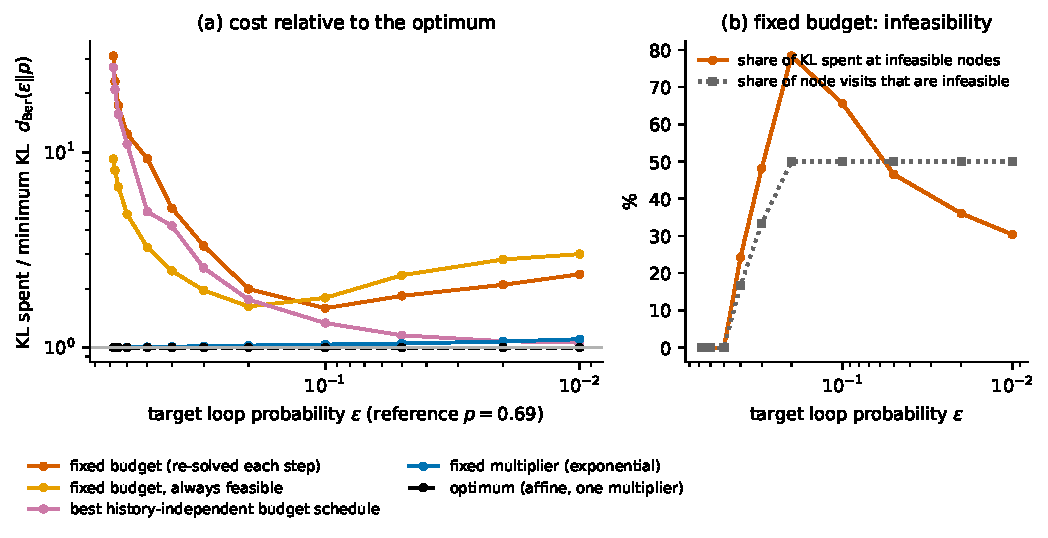
\includegraphics[width=\textwidth]{figures/fig_ladder.pdf}
\caption{Base system. (a) KL spent relative to the minimum KL for the same loop probability, for each rule of the ladder; the fixed price is within 10.3\% of the optimum throughout, the fixed budget is not. (b) Where the fixed-budget controller is infeasible: the share of node visits and the share of its KL spent at infeasible nodes.}\label{fig:ladder}
\end{figure}

\subsection{Infeasibility is not the explanation}\label{ssec:infeas}
A fixed budget is infeasible at a node when it lies below the floor $\min_v H(h,v)$, and Table~\ref{tab:ladder} shows that this affects 17--50\% of node visits at targets $\epsilon\le0.4$. The excess cannot be attributed to this alone, for three reasons.
\begin{enumerate}[leftmargin=*,itemsep=1pt]
\item \emph{The excess exists without any infeasibility.} At $\epsilon\ge0.5$ in the base system no node is infeasible, yet the fixed budget costs 9--31 times the minimum. In the persistent system with $R=3$ and $N=8$ no budget on the grid is infeasible at any target (0\% of node visits), and the fixed budget still costs 2.7--7.1 times the minimum.
\item \emph{Removing infeasibility does not remove the excess.} The always-feasible budget never collapses. It lowers the cost at weak control (12.4$\to$4.8 times at $\epsilon=0.6$) and raises it at strong control (2.4$\to$3.0 times at $\epsilon=0.01$), because with one fixed fraction of headroom at every node it still prices histories very differently ($1+\mathrm{CV}^2\approx11$, Table~\ref{tab:ladder}). Abstaining at infeasible nodes, the other way to avoid them, cannot reach any target below $\epsilon=0.4$ and costs more where it can (6.6 against 5.2 times at $\epsilon=0.4$).
\item \emph{What does remove it is a constant price.} The fixed-price rule has no budget to be infeasible, and its cost is within 12.5\% of the minimum.
\end{enumerate}
Infeasibility is a separate, additional cost that appears at strong control: at $\epsilon=0.2$, 78\% of the fixed-budget controller's KL is spent at nodes where its budget cannot be met. The universal mechanism, present at every target and in every system, is the allocation of distortion across histories.

\subsection{The waste law and its limit}\label{ssec:lawtest}
\begin{figure}[H]
\centering
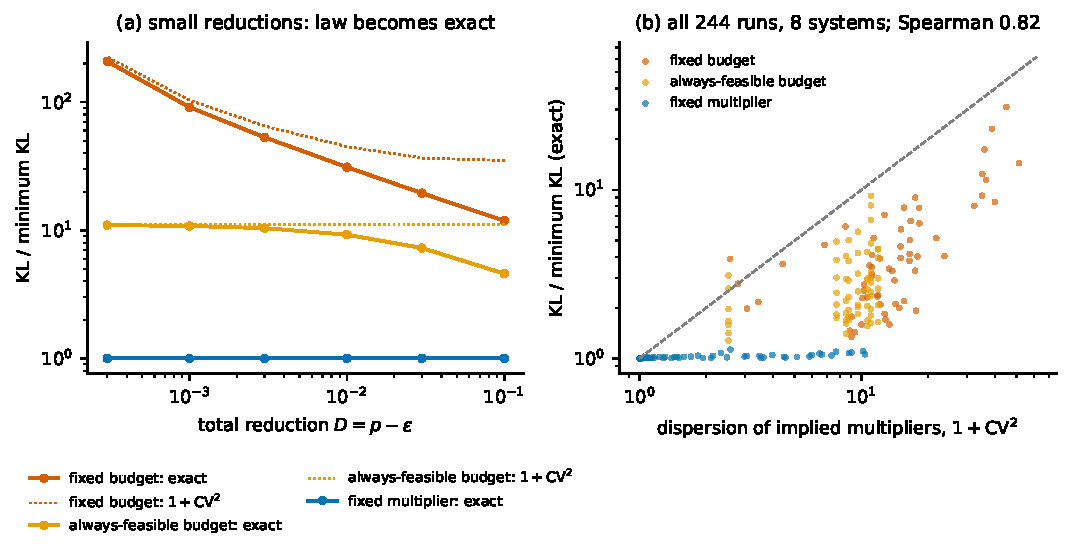
\includegraphics[width=\textwidth]{figures/fig_waste_law.pdf}
\caption{(a) Base system, small reductions $D=p-\epsilon$: exact cost ratio against the second-order prediction $1+\mathrm{CV}^2$. For the always-feasible budget the ratio reaches 0.99 of the prediction; for the fixed budget it rises in steps as fewer histories are touched and reaches the finite limit $1/\varphi_{\max}=707$ (dashed), at which only the single history of maximal hazard receives a reduction. The fixed price stays at 1. (b) All 244 runs of the eight systems: exact cost ratio against $1+\mathrm{CV}^2$ (Spearman $\rho=0.80$). The law over-predicts when the reduction is large, where the quadratic approximation no longer holds.}\label{fig:waste}
\end{figure}
\begin{table}[H]
\centering
\caption{Small reductions $D=p-\epsilon$ in the base system. Total path KL in bits of the minimum and of the fixed budget (FB), and cost ratios (exact KL as a multiple of the minimum) against the second-order prediction $1+\mathrm{CV}^2$ and, for FB, the second-order lower bound $1/\varphi$ of Proposition~\ref{prop:waste}. AF: always-feasible budget; FP: fixed price. As $D\to0$ the FB ratio tends to the finite limit $1/\varphi_{\max}=707.08$ (the single history of maximal hazard 0.991 is the only one touched, $\varphi_{\max}=0.00141$), while both costs tend to zero.}
\label{tab:smalld}
\resizebox{\textwidth}{!}{%
\begin{tabular}{@{}rrrrrrrrr@{}}
\toprule
 & & & \multicolumn{3}{c}{FB ratio} & \multicolumn{2}{c}{AF ratio} & FP \\
\cmidrule(lr){4-6}\cmidrule(lr){7-8}\cmidrule(lr){9-9}
$D$ & min KL & FB KL & exact & $1+\mathrm{CV}^2$ & $1/\varphi$ & exact & $1+\mathrm{CV}^2$ & exact \\
\midrule
0.1 & 3.21e-02 & 3.81e-01 & 11.9 & 35.1 & 30.1 & 4.58 & 11.04 & 1.0017 \\
0.03 & 2.98e-03 & 5.82e-02 & 19.5 & 36.7 & 30.1 & 7.27 & 11.04 & 1.0002 \\
0.01 & 3.35e-04 & 1.04e-02 & 31.1 & 45.0 & 34.4 & 9.23 & 11.04 & 1.0000 \\
0.003 & 3.03e-05 & 1.61e-03 & 53.2 & 65.1 & 53.6 & 10.39 & 11.04 & 1.0000 \\
0.001 & 3.37e-06 & 3.08e-04 & 91.4 & 103.6 & 58.4 & 10.81 & 11.04 & 1.0000 \\
0.0001 & 3.37e-08 & 1.15e-05 & 340.8 & 353.6 & 353.5 & 11.02 & 11.04 & 1.0000 \\
1e-05 & 3.37e-10 & 1.20e-07 & 354.5 & 355.9 & 353.5 & 11.04 & 11.04 & 1.0000 \\
1e-06 & 3.37e-12 & 1.98e-09 & 585.9 & 586.3 & 353.5 & 11.04 & 11.04 & 0.9991 \\
1e-07 & 3.37e-14 & 2.38e-11 & 707.0 & 707.1 & 707.1 & 10.95 & 11.04 & 0.9143 \\
\bottomrule
\end{tabular}}
\end{table}
Proposition~\ref{prop:waste} makes quantitative predictions that the exact computation can test (Figure~\ref{fig:waste}, Table~\ref{tab:smalld}). For small reductions the exact ratio $\KL/d_{\mathrm{Ber}}$ converges to $1+\mathrm{CV}^2$ (at $D=10^{-4}$ it is 0.998 of the prediction for the always-feasible budget and 0.96 for the fixed budget, and 1.00 for the fixed budget at $D=10^{-7}$), and the fixed-budget ratio rises as $D$ shrinks, but to a finite limit: when $D$ is small enough that only the history at the maximal hazard level (0.991) is touched, the second-order ratio equals $1/\varphi_{\max}=707.08$, with $\varphi_{\max}=0.00141$, and the exact ratio at $D=10^{-7}$ is 707.0. The ratio can be large while the absolute difference is negligible: at that point the fixed budget spends $2.4\cdot10^{-11}$ bits against a minimum of $3.4\cdot10^{-14}$ bits. At $D=0.1$ it spends 0.38 bits against 0.032.

The inequality $\KL/d_{\mathrm{Ber}}\ge1/\varphi$ is a statement about the second-order cost $K_2$ and holds for it exactly. For the exact KL it holds only approximately, and only near the second-order regime, because $\KL=K_2(1+o(1))$: the exact ratio exceeds $1/\varphi$ at three of the nine rows of Table~\ref{tab:smalld} ($D=10^{-3}$, $10^{-5}$, $10^{-6}$; for example 91 against 58 at $D=10^{-3}$) and is below it at the other six, by up to a factor of 2.5 at $D=0.1$ (11.9 against 30.1) and marginally at $D=10^{-4}$ (341 against 354) and $D=10^{-7}$ (707.0 against 707.1). Away from the second-order regime the law also overstates the waste (it predicts 35 where the exact ratio is 12), but it orders the controllers correctly: across all 244 runs the rank correlation between $\log(1+\mathrm{CV}^2)$ and the log of the exact ratio is 0.80. The dispersion of the implied prices, not the presence of infeasible steps, is what tracks the waste.

\subsection{Robustness}
\begin{table}[H]
\centering
\caption{Eight small systems. For each, the range over the target grid of the KL multiple (against the minimum) of the fixed budget (FB), the always-feasible budget (AF) and the fixed price (FP); the largest share of node visits at which the FB budget is infeasible; and the number of targets with no infeasible node. Targets are $p\times\{0.85,0.7,0.5,0.3,0.15,0.05,0.02\}$ (the base system uses the grid of Table~\ref{tab:ladder} and three near-reference targets). ``Persistent'': $R$ consecutive repeats are required for a loop.}
\label{tab:robust}
\resizebox{\textwidth}{!}{%
\begin{tabular}{@{}lrrrrrr@{}}
\toprule
System & $p$ & FB & AF & FP & max infeasible & targets with 0\% infeasible \\
\midrule
base (R=1, H=6) & 0.690 & 1.59--31.06 & 1.62--9.23 & 1.000--1.103 & 50\% & 5/12 \\
persistent R=2, H=6 & 0.355 & 1.59--9.00 & 2.19--5.65 & 1.000--1.019 & 33\% & 5/7 \\
persistent R=2, H=8 & 0.533 & 1.77--7.85 & 1.90--5.03 & 1.001--1.027 & 50\% & 5/7 \\
persistent R=3, H=8 & 0.424 & 2.74--7.11 & 1.79--4.95 & 1.000--1.011 & 0\% & 7/7 \\
rarer gateway (0.02) & 0.665 & 1.92--14.40 & 1.64--4.47 & 1.001--1.055 & 50\% & 2/7 \\
commoner gateway (0.10) & 0.756 & 1.34--7.82 & 1.40--4.05 & 1.003--1.096 & 50\% & 2/7 \\
weaker funnel (enter .5) & 0.684 & 1.70--11.49 & 1.55--4.28 & 1.002--1.082 & 67\% & 2/7 \\
temperature 0.8 & 0.651 & 1.97--6.06 & 1.27--3.11 & 1.001--1.125 & 67\% & 2/7 \\
\bottomrule
\end{tabular}}
\end{table}
Table~\ref{tab:robust} summarizes the ladder over eight systems. The ordering is the same in each: fixed price $\le$ always-feasible budget $\le$ fixed budget at weak control; the fixed price never exceeds 1.13 times the minimum, and the fixed budget never falls below 1.3. The persistent systems ($R=2,3$), whose events are closer to those of the text experiments, show the same pattern with smaller but still substantial waste (up to 9 times). What the exact systems do not contain is a language model: the hazard here is exact and the state space is small. Section~\ref{sec:real} asks which parts survive.

\section{A Qualified Test on a Language Model}\label{sec:real}

\subsection{Setup}
The primary model is an 848K-parameter, 4-layer, 128-dimensional character-level Transformer with a 256-character context, trained on Austen and Shelley (checkpoint \textsc{cosine}; Appendix~\ref{sec:protocol}). Every experiment uses the 15 \textsc{test} prompts (Appendix~\ref{app:prompts}), 10 seeds per prompt, generations of exactly 500 characters, and temperature $T=0.10$, a regime in which this model loops: in a 1000-character temperature sweep the loop rate falls from 96\% at $T=0.05$ to 0\% by $T=0.30$ (Appendix~\ref{sec:protocol}). The reference $P$ is plain temperature sampling at $T=0.10$. Recurrence risk uses $n$-gram orders 3--6. The loop event is the earliest position at which a span of length $P\in[2,60]$ repeats five times consecutively (a separate threshold of 8 for single-character runs). It is validated on seven held-out corpora with a pooled false-positive rate of 1.3\% (95\% CI [0.9\%, 1.9\%]), concentrated in one corpus (\emph{Dracula}, 8.7\%, epistolary formulas), and it is purely syntactic (Appendix~\ref{sec:event}); loop counts are counts of generations in which the detector fires, with that caveat attached. Decoders: the three recurrence-risk modes (Section~\ref{sec:setup}), repetition penalty (1.3), hard no-repeat 4-gram blocking, SuffixMatch ($\alpha=3$), and an FSD-style decoder and an LZ Penalty, both adapted from the published methods (Appendix~\ref{app:baselines}). Hard no-repeat blocking forbids the measured event by construction, so its zero loops are not a finding and it is excluded from every ranking and test (Appendix~\ref{ssec:hard-repeat}).

\subsection{Observed loop counts and per-step distortion}\label{ssec:common-kl}
\begin{table}[H]
\centering
\caption{Primary model (\textsc{cosine}), $T{=}0.10$, 15 test prompts $\times$ 10 seeds ($n{=}150$ each). Loops: generations in which the detector fires. $\KL(q\Vert p)$: per-step mean in bits against the common reference $p$ (multiply by 500 for the path KL of one generation); $\E_q[\mathrm{risk}]$: achieved recurrence risk under the same risk definition for every row. Sorted by KL. RMST, mcNLL and 4-gram similarity are in Table~\ref{tab:main}.}
\label{tab:primary}
\begin{tabular}{@{}lrrr@{}}
\toprule
Method & Loops & $\KL(q\Vert p)$ (bits) & $\E_q[\mathrm{risk}]$ \\
\midrule
Temperature 0.10 (reference) & 43/150 & 0.000 & 0.686 \\
\textsc{rr-fixed} ($\lambda{=}2$) & 4/150 & 0.037 & 0.550 \\
\textsc{rr-adaptive} & 0/150 & 0.096 & 0.466 \\
LZ Penalty (adapted) & 0/150 & 0.186 & 0.624 \\
Repetition penalty 1.3 & 7/150 & 0.388 & 0.533 \\
SuffixMatch ($\alpha{=}3$) & 0/150 & 0.436 & 0.285 \\
FSD-style (adapted) & 3/150 & 2.148 & 0.427 \\
No-repeat 4-gram$^{*}$ & 0/150 & 8.796 & 0.066 \\
\textsc{rr-dual} ($\varepsilon{=}0.05$) & 0/150 & 11.186 & 0.017 \\
\textsc{rr-dual} ($\varepsilon{=}0.01$) & 0/150 & 12.670 & 0.003 \\
\bottomrule
\end{tabular}

\vspace{4pt}
{\footnotesize $^{*}$Hard constraint on the measured event, so its zero loops are not a finding (Appendix~\ref{ssec:hard-repeat}). 95\% cluster CIs for KL and risk are within $\pm$6\% of the mean shown.}
\end{table}
Table~\ref{tab:primary} scores every decoder against the same reference and the same risk definition, by exposing each decoder's per-step distribution. The reference loops in 43 of 150 generations. Observed counts: \textsc{rr-dual} 0/150 at both $\varepsilon$ (95\% upper limit 2.4\%), \textsc{rr-adaptive} 0/150, LZ Penalty 0/150, SuffixMatch 0/150, FSD-style 3/150, \textsc{rr-fixed} 4/150, repetition penalty 7/150. These are counts at one temperature on one model, not guarantees. Per-step distortion differs by a factor of more than 100 among the decoders that reach zero observed loops (0.096 bits for \textsc{rr-adaptive} to 12.7 for \textsc{rr-dual}). The per-step guarantee of the dual mode held in every step (feasibility 100.0\%, zero maximum violation at the stored precision; Appendix~\ref{app:baselines}), so in this experiment the fixed-budget decoder is never infeasible, the situation of the $R=3$ system of Section~\ref{ssec:infeas}. RMST and paired comparisons are in Appendix~\ref{sec:protocol}: the exact test does not separate \textsc{rr-fixed} from the decoders with zero observed loops ($p=0.125$ at 15 prompts).

\subsection{A fixed price against a fixed budget}\label{ssec:frontier}
The theory suggests that a fixed-price rule should reach a given reduction of the loop probability at lower KL than a fixed-budget rule, and that the budget rule realizes widely varying prices. In the recurrence-risk decoder the two are the \textsc{fixed} mode (one $\lambda$ for the whole generation) and the \textsc{dual} mode (one $\varepsilon$ re-solved at every step). We sweep both on the same prompts, seeds, risk definition and detector, with $\lambda\in\{0.25,0.5,1,2,3,4,6,8,12\}$ and $\varepsilon\in\{1,0.95,0.9,0.85,0.8,0.75,0.7,0.65,0.6,0.5,0.3,0.2,0.1,0.05,0.01\}$, and record for every generation its loop event, its path KL and the per-step multiplier trace of the decoder. The budget $\varepsilon=1$ is a control: the constraint $\E_q[\mathrm{risk}]\le1$ is never active, so the dual mode must reproduce the reference decoder, which we check generation by generation. The comparison is descriptive: each setting has 75 generations, so an observed loop count does not establish equality of true loop probabilities, and we compare cost at similar observed counts with the intervals stated.

\begin{table}[H]
\centering
\caption{Primary model: fixed-price (recurrence-risk \textsc{fixed}) and fixed-budget (\textsc{dual}) rules at matched settings of the same sweep. Loops: generations with a detected loop. KL: path KL per 500-character generation, bits. Multiplier: mean (and, for the budget rule, mean / s.d.) of the per-step multiplier $\lambda_t$ realized over the generation, in nats of risk. $\lambda_t=0$: share of steps at which the budget constraint was inactive.}
\label{tab:frontier}
\begin{tabular}{@{}lrrrr@{}}
\toprule
Rule & Loops & Path KL (bits) & Multiplier & $\lambda_t=0$ \\
\midrule
reference (T=0.10) & 29/75 & 0.0 & --- & 0\% \\
fixed price, $\lambda{=}0.25$ & 15/75 & 0.3 & 0.2 & 0\% \\
fixed price, $\lambda{=}0.5$ & 9/75 & 1.2 & 0.5 & 0\% \\
fixed price, $\lambda{=}1$ & 4/75 & 5.0 & 1.0 & 0\% \\
fixed price, $\lambda{=}2$ & 2/75 & 18.5 & 2.0 & 0\% \\
fixed price, $\lambda{=}3$ & 0/75 & 38.6 & 3.0 & 0\% \\
fixed price, $\lambda{=}4$ & 1/75 & 63.8 & 4.0 & 0\% \\
fixed price, $\lambda{=}6$ & 0/75 & 121.3 & 6.0 & 0\% \\
fixed price, $\lambda{=}8$ & 0/75 & 178.8 & 8.0 & 0\% \\
fixed price, $\lambda{=}12$ & 0/75 & 277.3 & 12.0 & 0\% \\
fixed budget, $\varepsilon{=}1$ & 29/75 & 0.0 & 0.0 / 0.1 & 100\% \\
fixed budget, $\varepsilon{=}0.95$ & 0/75 & 457.8 & 13.1 / 23.1 & 60\% \\
fixed budget, $\varepsilon{=}0.9$ & 0/75 & 730.3 & 10.5 / 21.1 & 67\% \\
fixed budget, $\varepsilon{=}0.85$ & 0/75 & 880.2 & 8.4 / 19.2 & 72\% \\
fixed budget, $\varepsilon{=}0.8$ & 0/75 & 1044.2 & 7.5 / 18.2 & 75\% \\
fixed budget, $\varepsilon{=}0.75$ & 0/75 & 1057.4 & 6.1 / 16.5 & 79\% \\
fixed budget, $\varepsilon{=}0.7$ & 0/75 & 1209.3 & 8.8 / 20.6 & 73\% \\
fixed budget, $\varepsilon{=}0.65$ & 0/75 & 1355.7 & 8.3 / 20.4 & 75\% \\
fixed budget, $\varepsilon{=}0.6$ & 0/75 & 1477.7 & 7.9 / 20.4 & 77\% \\
fixed budget, $\varepsilon{=}0.5$ & 0/75 & 1696.0 & 7.3 / 20.3 & 80\% \\
fixed budget, $\varepsilon{=}0.3$ & 0/75 & 2588.2 & 13.5 / 32.4 & 76\% \\
fixed budget, $\varepsilon{=}0.2$ & 0/75 & 3494.2 & 36.3 / 67.7 & 60\% \\
fixed budget, $\varepsilon{=}0.1$ & 0/75 & 4812.9 & 38.7 / 78.2 & 65\% \\
fixed budget, $\varepsilon{=}0.05$ & 0/75 & 5641.9 & 39.2 / 80.4 & 67\% \\
fixed budget, $\varepsilon{=}0.01$ & 0/75 & 6363.6 & 40.5 / 82.7 & 68\% \\
\bottomrule
\end{tabular}
\end{table}
\begin{figure}[H]
\centering
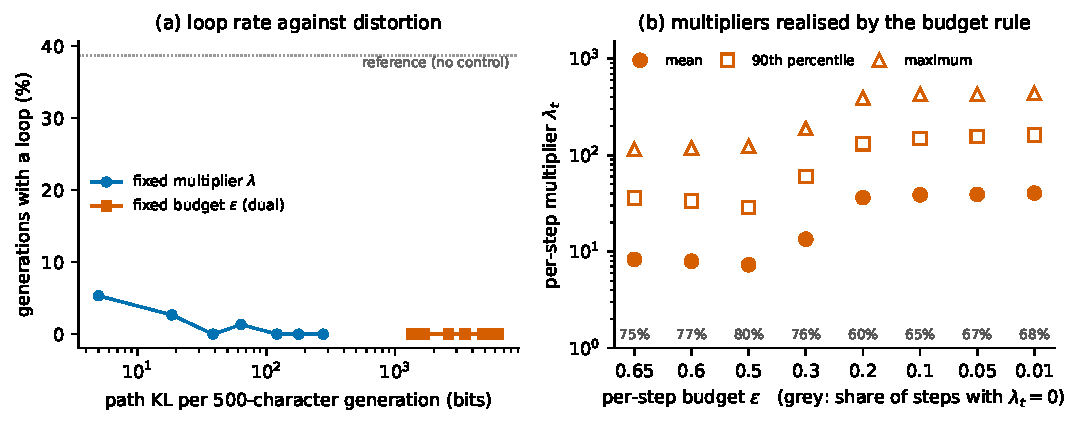
\includegraphics[width=\textwidth]{figures/fig_frontier.pdf}
\caption{Primary model, $T=0.10$, 75 generations per setting. (a) Share of generations with a detected loop against the path KL per 500-character generation, for the fixed-price rule (one $\lambda$ for the whole generation) and the fixed-budget rule (one $\varepsilon$ re-solved at every step); the budget $\varepsilon=1$ (no active constraint) coincides with the reference and has zero KL. (b) Per-step multipliers $\lambda_t$ that the budget rule realizes for $\varepsilon<1$: mean, 90th percentile and maximum over steps, and the share of steps at which the constraint is inactive ($\lambda_t=0$).}\label{fig:frontier}
\end{figure}
Table~\ref{tab:frontier} and Figure~\ref{fig:frontier} give the sweep (75 generations per setting, seeds 1--5 of the 15 prompts; the reference loops in 29 of them). The control behaves as it should: the budget $\varepsilon=1$ reproduces the reference generation by generation (75 of 75 generations have the same loop onset, total KL $\le6\cdot10^{-6}$ bits). The two families then differ sharply. The fixed price moves smoothly with $\lambda$: 15/75 loops at 0.3 bits ($\lambda=0.25$), 9/75 at 1.2 bits, 4/75 at 5.0 bits, 2/75 at 18.5 bits (4/150 in the full run of Table~\ref{tab:primary}) and 0/75 at 38.6 bits ($\lambda=3$). The budget rule has no setting with an intermediate count on this grid: the count drops from 29/75 at $\varepsilon=1$ to 0/75 at $\varepsilon=0.95$, at 458 bits, and stays at 0/75 for every tighter budget, at 458 to 6364 bits (cost rising as the budget tightens). Among settings with zero observed loops the cheapest budget costs 12 times the cheapest fixed price ($\lambda=3$; prompt-bootstrap 95\% interval 11--12) and 25 times the fixed price with 2/75 loops; the tightest costs 165 times ($\lambda=3$, interval 156--174) and 23 times the strongest fixed price tested ($\lambda=12$, 277 bits). This is a comparison of cost at similar \emph{observed} counts. A count of 0/75 has a 95\% upper limit of 4.8\% on the true rate, so it does not show that two settings have equal loop probabilities; for that, the count of the budget rule would have to be resolved between $\varepsilon=0.95$ and 1, a range of the grid that was not subdivided further.

The multipliers explain the cost, as in Section~\ref{sec:small}. Wherever the budget rule is active ($\varepsilon<1$), the constraint is inactive ($\lambda_t=0$) at 60--80\% of steps, and where it acts it uses large multipliers: a 90th percentile of 26--163 and a maximum of 94--437 (mean over generations, Figure~\ref{fig:frontier}b), against a single $\lambda$ of 0.25--12 for the fixed-price rules. The price of risk it pays varies by two orders of magnitude within a generation, which is the dispersion that Proposition~\ref{prop:waste} identifies with excess cost. Two limits apply. The recurrence risk is a proxy and not the hazard, so the quantitative law is not tested here; and the average reference risk of about 0.69 is not the point at which the constraint becomes inactive, which is why the sweep extends to $\varepsilon=1$.


\subsection{How much of the path KL moves the loop probability}\label{ssec:eventlevel}
Section~\ref{ssec:bernoulli-bound} splits a decoder's path divergence into the term $d_{\mathrm{Ber}}(Q(E)\Vert P(E))$ needed to move the loop probability and a remainder, the distortion of the conditional shape of the generation. We estimate both for every decoder from the sample-level records of the run behind Table~\ref{tab:primary} (for each generation: its prompt, loop event and total path KL).

\textbf{The comparison is conditioned on the prompt.} The decomposition applies prompt by prompt, $\KL(Q_x\Vert P_x)\ge d_{\mathrm{Ber}}(Q_x(E)\Vert P_x(E))$, and the quantities reported are averages over the 15 prompts with weights $1/15$. Pooling the prompts first would use the pooled loop rates and, by joint convexity of $d_{\mathrm{Ber}}$, can only lower the bound, overstating the distortion that is not needed; the reference loop count differs by prompt (1 to 6 of 10 generations), but the difference is small here (at a decoder loop fraction of zero the plug-in event term is 0.528 bits prompt by prompt and 0.487 bits pooled). $P_x(E)$ and $Q_x(E)$ are loop fractions over the 10 seeds of one prompt; the plug-in $d_{\mathrm{Ber}}$ is infinite whenever a fraction is 0 or 1 and the other is not, so the primary estimate smooths both fractions as $(k+\tfrac12)/(n+1)$, with plug-in and Laplace ($(k+1)/(n+2)$) smoothings as a sensitivity range. Intervals are percentile intervals from resampling whole prompts (10{,}000 resamples), which keeps each generation's loop event and path KL together. Everything is a sample estimate from 150 generations per decoder; it is descriptive and has no guaranteed coverage.

\begin{table}[H]
\centering
\caption{Prompt-conditional decomposition of total path KL (bits per generation of 500 characters) into the event term $\frac1{15}\sum_x d_{\mathrm{Ber}}(\tilde Q_x(E)\Vert\tilde P_x(E))$ and the remainder (excess), primary model, $T{=}0.10$, 150 generations per decoder. Brackets are 95\% percentile intervals from resampling the 15 prompts. A tilde marks Jeffreys-smoothed loop fractions over 10 seeds; ``range'' gives the event term under Laplace, Jeffreys and plug-in fractions. Descriptive plug-in estimates, not bounds with guaranteed coverage.}
\label{tab:pcb}
\resizebox{\textwidth}{!}{%
\begin{tabular}{@{}lrrrrr@{}}
\toprule
Method & Loops & Path KL & Event term & Range & Excess \\
\midrule
\textsc{rr-fixed} & 4/150 & 18.6 [18.2, 19.0] & 0.30 [0.16, 0.46] & 0.23--0.44 & 18.3 [17.9, 18.7] \\
\textsc{rr-adaptive} & 0/150 & 48.2 [46.6, 49.7] & 0.35 [0.22, 0.51] & 0.27--0.53 & 47.8 [46.2, 49.4] \\
LZ Penalty (adapted) & 0/150 & 92.8 [90.2, 95.6] & 0.35 [0.22, 0.51] & 0.27--0.53 & 92.4 [89.8, 95.2] \\
Repetition penalty 1.3 & 7/150 & 194.1 [183.9, 205.7] & 0.26 [0.13, 0.41] & 0.20--0.37 & 193.9 [183.6, 205.5] \\
SuffixMatch ($\alpha{=}3$) & 0/150 & 217.8 [214.5, 221.0] & 0.35 [0.22, 0.50] & 0.27--0.53 & 217.4 [214.2, 220.6] \\
FSD-style (adapted) & 3/150 & 1074.2 [1039.5, 1109.1] & 0.32 [0.18, 0.48] & 0.25--0.46 & 1073.9 [1039.1, 1108.9] \\
No-repeat 4-gram & 0/150 & 4397.9 [4329.7, 4462.7] & 0.35 [0.22, 0.51] & 0.27--0.53 & 4397.6 [4329.5, 4462.3] \\
\textsc{rr-dual} ($\varepsilon{=}0.05$) & 0/150 & 5593.2 [5524.1, 5662.2] & 0.35 [0.22, 0.51] & 0.27--0.53 & 5592.8 [5523.7, 5661.9] \\
\textsc{rr-dual} ($\varepsilon{=}0.01$) & 0/150 & 6334.8 [6226.6, 6441.4] & 0.35 [0.22, 0.51] & 0.27--0.53 & 6334.5 [6226.1, 6441.1] \\
\bottomrule
\end{tabular}}
\end{table}
For every decoder the estimated event term lies between 0.20 and 0.53 bits under all three smoothings, whereas the measured path KL ranges from 19 to over 6000 bits (Table~\ref{tab:pcb}). At least 98\% of what each decoder spends is estimated to be distortion of the conditional shape of the generation and not the cost of moving the loop probability: 98.4\% for \textsc{rr-fixed}, above 99.9\% for FSD-style, no-repeat blocking and \textsc{rr-dual}. The event term itself is uncertain by about $\pm0.15$ bits because it rests on 10 generations per prompt, which does not affect this reading.

\textbf{What this does and does not say.} The excess is measured against the cost of moving the loop probability by reweighting whole sequences by whether they loop. That bound is attained only by a rule that has the hazard at every step, or by rejecting whole generations; Section~\ref{sec:small} shows that even with the exact hazard a fixed budget spends multiples of it. The excess of a decoder is therefore not a saving available to that decoder, and we do not claim that 98\% of any decoder's distortion could be removed. The estimate rules out one reading, that the large KL of the heavy decoders is spent on lowering the loop probability, and it says nothing about text quality.

\subsection{What transfers and what remains a hypothesis}\label{ssec:transfer}
\begin{table}[H]
\centering
\caption{Findings of the exact systems against the language-model evidence.}
\label{tab:transfer}
\small
\begin{tabular}{@{}p{0.27\linewidth}p{0.45\linewidth}p{0.20\linewidth}@{}}
\toprule
Finding in the exact systems & Language-model evidence & Status \\
\midrule
A fixed budget spends far more KL than the minimum for the loop probability it reaches & Every decoder, \textsc{rr-dual} included, spends at least 98\% of its path KL beyond the event term (Table~\ref{tab:pcb}) & Consistent; no saving is shown \\
At equal loop rate a fixed price is cheaper than a fixed budget & Sweep of Section~\ref{ssec:frontier} (Figure~\ref{fig:frontier}, Table~\ref{tab:frontier}) & Supported at similar observed loop counts (budget rule jumps from reference level to 0/75 between $\varepsilon=1$ and 0.95) \\
A fixed budget realizes widely varying prices & Per-step multiplier traces of \textsc{rr-dual} (Table~\ref{tab:frontier}) & Supported (descriptive; proxy risk) \\
The waste does not need infeasible steps & \textsc{rr-dual} is feasible at 100\% of steps on every model (Appendix~\ref{sec:generalization}) & Supported for the recurrence-risk proxy \\
With the exact hazard a causal rule attains the optimum & A rollout estimate separates risky from novel candidates; no decoder is built on it (Appendix~\ref{sec:hazard-transfer}) & Hypothesis \\
The quantitative waste law & Needs the hazard as risk signal, which is not available & Hypothesis \\
Rejection of looping samples attains the bound when streaming is not needed & Cost of 0.49 bits and 1.4 generations computed from the loop rate; not run end to end & Computed, not tested \\
\bottomrule
\end{tabular}
\end{table}
The prompt-conditional analysis was run on the primary model only, the only model for which sample-level path KL is stored. The other models (a character model trained on non-fiction, GPT-2, OLMo-2-0425-1B, Mistral-7B-v0.3; Appendix~\ref{sec:generalization}) are compared at a compact scale and show that the heuristics' effectiveness varies from model to model: \textsc{rr-fixed} has 4/150 loops on the primary model and 77/150 on the non-fiction model, and the LZ Penalty and the FSD-style decoder reach zero observed loops on some models and not on others. The dual mode's per-step feasibility was exactly 100.0\% on every model. Qwen2.5-3B showed no repetition regime at the budget tested and is not compared.

\section{Discussion}\label{sec:discussion}

\subsection{What is established}
In exactly solvable systems, the loss of a fixed per-step risk budget is a loss of allocation. The probability of a loop falls by the visit-weighted sum of per-step hazard reductions (Proposition~\ref{prop:accounting}); the cheapest allocation holds the price of risk constant (Proposition~\ref{prop:waste}); a fixed budget instead implies prices that vary by orders of magnitude, and its excess cost tracks their dispersion; and a fixed price recovers the optimum to within 12.5\% in all eight systems tested. The optimum itself is a causal rule, so per-step control is not inefficient because it is causal. It is inefficient when it holds the wrong quantity fixed.

\subsection{How to read the numbers}
\begin{itemize}[leftmargin=*,itemsep=2pt]
\item \textbf{Zero observed loops is not a guarantee.} Every zero is a count of a syntactic detector firing in 50--150 generations at one temperature; with 150 generations the 95\% upper limit for a true rate is 2.4\%. The dual mode's guarantee is local: it bounds the expected recurrence risk at each step when the numerical projection succeeds, and it does not bound the probability of a loop.
\item \textbf{KL is distortion, not text quality.} A pilot human evaluation (Appendix~\ref{sec:human-eval}, $n=9$) found no reliable readability difference among four decoders whose per-step KL differs by a factor of about 70; it neither supports nor contradicts a cost of distortion.
\item \textbf{The 98\% excess is not a saving.} It is distance from a benchmark that needs the hazard (Section~\ref{ssec:eventlevel}).
\end{itemize}

\subsection{Alternatives to streaming control}\label{ssec:alternatives}
When generation need not be streamed, rejecting a whole generation in which the detector fires and drawing a new one attains the event-level optimum at $Q(E)=0$ exactly: at the primary model's reference loop rate of 28.7\% it costs 0.49 bits and 1.4 generations per accepted sample, against 19--6300 bits per generation for the decoders of Table~\ref{tab:pcb}. Its cost grows as $1/(1-p)$, so it is unattractive when almost every generation loops (greedy decoding loops in 140 of 150), it needs a detector that can be evaluated on a completed generation, and it samples from the model conditioned on the detector not firing, which is only as good as the detector. Sequence-aware causal control with an estimated hazard is the streaming counterpart; a rollout estimate of the hazard separates risky from novel candidates (Appendix~\ref{sec:hazard-transfer}), but turning it into a calibrated per-step rule is not attempted here.

\subsection{Limitations}
\begin{itemize}[leftmargin=*,itemsep=2pt]
\item \textbf{Exact systems are small.} The hazard is exact and the state space has 20 states; eight variants support robustness but are not a language model.
\item \textbf{The theory is second order.} Proposition~\ref{prop:waste} is exact algebra and an asymptotic statement about cost; at large reductions it over-predicts (Figure~\ref{fig:waste}). It is stated for the hazard as risk signal; the recurrence-risk proxy of the language-model experiments is not the hazard, so the quantitative law is not claimed there.
\item \textbf{One temperature, one primary model.} $T=0.10$, 15 prompts, 10 seeds on an 848K-parameter model; the other models are compared at 50--150 generations per configuration with no sample-level KL records.
\item \textbf{Detector.} The pooled false-positive rate of about 1.3\% conceals per-corpus variance (\emph{Dracula}: 26/300, about seven times the pooled figure); the calibration of the subword detectors did not meet the pre-declared 1\% tolerance (Appendix~\ref{sec:generalization}); the detector does not capture semantic repetition.
\item \textbf{Baselines.} FSD-style and LZ Penalty are adapted from the published methods and are not reproductions (Appendix~\ref{app:baselines}); SuffixMatch is our own heuristic.
\item \textbf{Units and tolerances.} All KL values are in bits and all per-step values are means over the fixed generation length; solver tolerances, float32 computation and exact-computation residuals are stated in Appendix~\ref{app:baselines}.
\end{itemize}

\section{Conclusion}\label{sec:conclusion}
A fixed per-step risk budget can waste KL when the goal is to prevent a loop anywhere in a sequence, because it fixes the level of one-step risk rather than its price. The loop probability falls by the sum of per-step hazard reductions, the cheapest allocation keeps the price constant, and a fixed budget instead prices histories very differently; to second order its excess cost is one plus the squared coefficient of variation of those prices. In exact systems a fixed price stays within 12.5\% of the minimum KL while a fixed budget costs 1.3 to about 700 times as much (the largest ratios at the smallest reductions, where both costs are negligible in bits), with and without infeasible budgets. On a character-level language model the same ordering appears descriptively: a fixed price reached zero observed loops at 39 bits per generation, every fixed budget below 1 that was tested cost at least 458 bits, and the budget rule realized multipliers that were zero at most steps and in the hundreds at others. What remains open is a sequence-aware causal decoder for real text, which needs an estimate of the event-to-go hazard; when streaming is not needed, rejection of loop-containing samples already attains the optimum for the event the detector defines.


\vspace{6pt}
\authorcontributions{The author defined the research question, ran the language-model experiments, collected the human-evaluation responses, reviewed and verified the results and is responsible for the content. A generative AI assistant helped with the implementation of code and tests, the preparation of figures and tables from saved results, and the drafting and editing of the text; the author reviewed all of it.}
\funding{This research received no external funding.}
\institutionalreview{No institutional ethical review was sought. The pilot human evaluation of Appendix~\ref{sec:human-eval} was a short anonymous task in which volunteers judged machine-generated text; no sensitive personal data were collected, and the released result files identify participants only by the labels they chose.}
\informedconsent{Participants were told the nature and length of the task on the introduction page of the evaluation tool before taking part; no written consent was collected.}
\dataavailability{Code, tests, saved results and the scripts that generate every table are available at https://github.com/inopolis/GAI-project (release tag \texttt{paper-final}); see Appendix~\ref{sec:reproducibility}.}
\acknowledgments{A generative AI assistant was used as a support tool for implementing code and tests, preparing figures and tables from saved results, and drafting and editing text. The mathematical statements are accompanied by numerical checks in the released tests (Appendix~\ref{sec:reproducibility}); the author reviewed the assistant's output and is responsible for the correctness of the mathematics, the results and the final text.}
\conflictsofinterest{The author declares no conflict of interest.}

\appendixtitles{yes}
\appendixstart
\appendix
\section{Proofs}\label{app:proofs}

\textbf{Proposition~\ref{prop:min}.} Equation~\eqref{eq:decomp} is the chain rule $\KL(Q\Vert P)=\KL(Q_Z\Vert P_Z)+\E_{Z\sim Q}\KL(Q_{X|Z}\Vert P_{X|Z})$ for the coarse-graining $X\mapsto Z=\mathbf{1}[E]$. The conditional terms are non-negative and vanish for $Q(\cdot\mid E)=P(\cdot\mid E)$ and $Q(\cdot\mid E^c)=P(\cdot\mid E^c)$. With $Q(E)=\epsilon$ this leaves $\KL(Q\Vert P)\ge d_{\mathrm{Ber}}(\epsilon\Vert p)$ with equality exactly for $Q^\star(x)=P(x)\epsilon/p$ on $E$ and $P(x)(1-\epsilon)/(1-p)$ off $E$.

\textbf{Proposition~\ref{prop:causal}.} The ratio of $Q^\star/P$ on $E$ to that off $E$ is $\epsilon(1-p)/[p(1-\epsilon)]=2^{-\lambda}$, so $Q^\star(x)\propto P(x)2^{-\lambda\mathbf{1}[x\in E]}$. Marginalizing sequentially, the transition of $Q^\star$ at a history $h$ is proportional to $P(v\mid h)\,\E_P[2^{-\lambda\mathbf{1}[E]}\mid h,v]=P(v\mid h)[1-(1-2^{-\lambda})H(h,v)]$.

\textbf{Proposition~\ref{prop:accounting}.} Let $V(h)=\sum_vp(v\mid h)H(h,v)$ for a history that has not looped, with $V=0$ at the horizon, and $\Phi_t=\mathbf{1}[\text{looped by }t]+\mathbf{1}[\text{not looped by }t]V(h_t)$. Then $\Phi_0=P(E)$, $\Phi_N=\mathbf{1}[E]$, and under a Markov controller $\E_Q[\Phi_{t+1}-\Phi_t\mid h_t]=\sum_vq(v\mid h_t)H(h_t,v)-V(h_t)=-\Delta(h_t)$ for $h_t$ not yet looped. Summing over $t$ and taking expectations gives (a). For (b), $\Phi_t$ is a martingale under $P$ with $\Phi_0=p$ and $\Phi_N=\mathbf{1}[E]$, so $p(1-p)=\mathrm{Var}(\mathbf{1}[E])=\sum_t\E_P[\mathrm{Var}(\Phi_{t+1}\mid h_t)]$, and for a history that has not looped $\mathrm{Var}(\Phi_{t+1}\mid h_t)=\sigma^2(h_t)$.

\textbf{Proposition~\ref{prop:waste}.} Tilting $p$ by $e^{-\lambda H}$ gives $\Delta=\lambda\sigma^2+O(\lambda^2)$ and $\KL=\frac{\lambda^2\sigma^2}{2\ln2}+O(\lambda^3)$ bits, hence $\KL=\Delta^2/(2\sigma^2\ln2)\,(1+o(1))$ as $\Delta/\sigma\to0$ (iii). For (i), Cauchy--Schwarz gives $D^2=\big(\sum_h(\sqrt{w_P}\Delta/\sigma)(\sqrt{w_P}\sigma)\big)^2\le\big(\sum_hw_P\Delta^2/\sigma^2\big)\big(\sum_hw_P\sigma^2\big)=2\ln2\,K_2\,p(1-p)$, using Proposition~\ref{prop:accounting}(b); equality holds iff $\Delta/\sigma\propto\sigma$, i.e.\ $\lambda_h$ constant, and then $K_2=D^2/(2\ln2\,p(1-p))$, which is the second-order expansion of $d_{\mathrm{Ber}}(p-D\Vert p)$. For (ii), with $u_h=\Delta/\sigma^2=\lambda_h$ and $\pi_h=w_P\sigma^2/(p(1-p))$ one has $D=p(1-p)\,\E_\pi[u]$ and $\sum w_P\Delta^2/\sigma^2=p(1-p)\,\E_\pi[u^2]$, so $K_2/K^\star=\E_\pi[u^2]/\E_\pi[u]^2=1+\mathrm{CV}^2$. Restricting the Cauchy--Schwarz inequality to the touched set $A$ gives $\E_\pi[u]^2\le\varphi\,\E_\pi[u^2]$, hence $K_2/K^\star\ge1/\varphi$. The weights $w_P$ are used in place of $w_Q$; they differ by a relative $O(D)$, which does not change the leading order.

\section{Loop-Event Validation}
\label{sec:event}
%==============================================================================

\subsection{Why the naive event fails}
\label{ssec:naive-fails}
The candidate event ``the first repeated $n$-gram of length $n$'' fires on 54.0\% of held-out Doyle windows and 72.0\% of held-out Dickens windows at $n{=}10$. An event that fires on the majority of ordinary prose cannot distinguish degeneration from fluency and is not used.

\subsection{Calibration}
The persistent-cycle event is the earliest position $e$ at which a span of length $P\in[2,P_{\max}]$ repeats exactly $R$ times consecutively. $R$ and $P_{\max}$ are chosen by a pre-declared rule (the smallest $R$ whose worst-case upper 95\% CI, across window lengths 300/500/1000/2000, falls at or below a 1\% tolerance) on a calibration set (Carroll, Twain, Swift) never referenced afterward. No cell meets the 1\% tolerance at every window length; $R{=}6$ reproduces $R{=}5$'s counts exactly, indicating that the residual is stable and not a threshold-boundary artifact. Frozen: $R{=}5$, $P_{\max}{=}60$, with worst-case upper CI 2.80\%, which does not meet the a priori target.

Period 1 (a single repeated character) uses a separate, decoupled threshold of 8. Using $R{=}5$ for period 1 caused plain-text typesetting conventions (five-character dash dividers) to fire; the threshold of 8 sits above ordinary divider and ellipsis lengths and below observed degenerate runs. Every other period $P\in[2,60]$ uses $R{=}5$.

\subsection{Validation battery}
\begin{table}[H]
\centering
\caption{Validation battery for the frozen event.}
\label{tab:validation}
\begin{tabular}{@{}lrrl@{}}
\toprule
Corpus & fires/$n$ & rate & 95\% CI \\
\midrule
Melville, \emph{Moby-Dick}      & 0/300  & 0.0\% & [0.0\%, 1.2\%] \\
Stoker, \emph{Dracula}          & 26/300 & 8.7\% & [5.7\%, 12.4\%] \\
Whitman, \emph{Leaves of Grass} & 0/300  & 0.0\% & [0.0\%, 1.2\%] \\
Paine, \emph{Common Sense}      & 1/249  & 0.4\% & [0.0\%, 2.2\%] \\
Homer, \emph{Iliad} (trans.)    & 0/300  & 0.0\% & [0.0\%, 1.2\%] \\
Doyle, \emph{Sherlock Holmes}   & 0/300  & 0.0\% & [0.0\%, 1.2\%] \\
Dickens, \emph{A Tale of Two Cities} & 0/300 & 0.0\% & [0.0\%, 1.2\%] \\
\midrule
\textbf{Pooled}                 & 27/2049 & \textbf{1.3\%} & \textbf{[0.9\%, 1.9\%]} \\
\bottomrule
\end{tabular}
\end{table}
The residual is concentrated almost entirely in \emph{Dracula} (epistolary formulas); poetry (Whitman) shows zero false positives. Robustness to window length (300/500/1000/2000 characters) gives 0.0\%/0.5\%/1.4\%/2.4\%.

\subsection{Synthetic sensitivity}
Constructed text with a known period $P\in\{1,\allowbreak2,\allowbreak3,\allowbreak5,\allowbreak8,\allowbreak13,\allowbreak20,\allowbreak30,\allowbreak45,\allowbreak60\}$ repeated $R_{\text{true}}\in\{2,\allowbreak3,\allowbreak4,\allowbreak5,\allowbreak8,\allowbreak10\}$ times is detected correctly in 98--100\% of cases at every tested repeat count.



\section{Experimental Protocol and Additional Primary-Model Results}
\label{sec:protocol}

\subsection{Model and data}
The primary model is an 848K-parameter, 4-layer, 128-dimensional character-level Transformer with a 256-character context, trained on Austen and Shelley, validated on Doyle, and tested on Dickens. All primary-model results use the \textsc{cosine}-schedule checkpoint unless stated otherwise. A second, independently trained checkpoint of the same architecture and data (\textsc{baseline}, constant learning rate) provides a replication: greedy decoding loops at 60.0\% (vs.\ 93.3\% for \textsc{cosine}) and $T{=}0.15$ still shows a 4.0\% loop rate where \textsc{cosine} shows 0.0\%, so the temperature threshold does not carry over even across retrains of the same architecture and data. \textsc{rr-dual} ($\varepsilon{=}0.05$) reaches 0/150 loops on \textsc{baseline} at 100.0\% feasibility and 11.343 bits of KL, close to \textsc{cosine}'s 11.186 bits (Table~\ref{tab:main}).

\subsection{Where the pathology occurs}
A sweep of 14 temperatures $\times$ 5 prompts $\times$ 10 seeds (1000-character generations, exact Clopper--Pearson intervals) shows the loop rate falling smoothly from 96.0\% at $T{=}0.05$ to 0.0\% by $T{=}0.30$, crossing below 5\% near $T{\approx}0.2$. Every primary-model decoding comparison runs at $T{=}0.10$. The sweep was not repeated for the second model (Section~\ref{sec:generalization}), whose safe temperature range does not simply transfer.

\subsection{Prompt protocol}
A \textsc{Dev} set of 5 prompts is the only material inspected while choosing hyperparameters. A disjoint \textsc{Test} set of 15 prompts, written afterward and not inspected during tuning, is the source of every number in Sections~\ref{ssec:common-kl} and~\ref{sec:generalization}. All configurations, greedy decoding included, are evaluated on all 15 test prompts.

\subsection{Inference}
\label{ssec:inference}
The unit of analysis for every confidence interval and hypothesis test is the \emph{prompt}. Two procedures were declared in advance:
\begin{itemize}[leftmargin=*]
  \item \textbf{Primary: exact sign-flip test.} For 15 prompts, all $2^{15}$ sign patterns are enumerated, giving an exact $p$-value for the paired difference in prompt-level RMST (\texttt{compute\_\allowbreak{}significance.py}, which reproduces every number in Table~\ref{tab:paired}).
  \item \textbf{Sensitivity: cluster bootstrap.} 3000 resamples of prompts give a 95\% CI for the same statistic.
\end{itemize}
At small $n$ the two need not agree; Section~\ref{ssec:disagreement} reports where they differ. The primary test governs.

\subsection{Metrics}
\textbf{RMST} has a horizon of 500 characters and uses Kaplan--Meier with right-censoring. Model-consistency NLL (mcNLL) scores every target position independently with its exact context window $\text{full}[\max(0,t{-}\text{block\_size}):t]$, batched with right-padding so that causal masking cannot leak filler into real positions (Appendix~\ref{app:defects}). 4-gram similarity is measured against a held-out reference corpus. For dual-calibrated configurations the exact $\KL(q\Vert p)$, achieved risk, and per-step feasibility diagnostics are reported. Every $\KL(q\Vert p)$ figure reported anywhere in this paper for a real model, including Tables~\ref{tab:main}, \ref{tab:primary}, \ref{tab:olmofull}, and \ref{tab:mistralfull}, is a \emph{per-step mean}: the divergence $\KL(q_t\Vert p_t)$ between that step's sampling distribution and the shared reference is computed at every generated position, averaged over the fixed generation length of that sample (500 characters for the primary and non-fiction models, 200 tokens for GPT-2, 150 for OLMo and Mistral), and then averaged again over samples. Generation always runs for the full fixed length regardless of whether or when a loop is detected, so a sample's total path divergence is exactly its reported per-step mean multiplied by that fixed length.

\subsection{No-repeat blocking is excluded from ranking}
\label{ssec:hard-repeat}
A global no-repeat-$n$-gram filter, checked against the entire history, structurally cannot sustain a persistent cycle of any period $P$: once a period-$P$ cycle has run for at least $n$ steps, every subsequent $n$-gram repeats one produced $P$ steps earlier and is blocked, regardless of the relation between $P$ and $n$. Its 0/150 result holds by construction and is not an experimental finding, so it is excluded from every significance test and from the survival ranking.

\subsection{Paired comparisons}
\label{ssec:disagreement}
\begin{table}[H]
\centering
\caption{Paired, prompt-clustered comparisons of RMST (\texttt{compute\_\allowbreak{}significance.py}).}
\label{tab:paired}
\resizebox{\textwidth}{!}{%
\begin{tabular}{@{}lrrl@{}}
\toprule
Comparison ($A-B$) & $\Delta$RMST & $p$ (exact) & 95\% cluster CI \\
\midrule
\textsc{rr-fixed} $-$ Temperature 0.10   & $+88.4$  & $<0.001$ & [66.4, 113.9] \\
\textsc{rr-fixed} $-$ Rep.\ penalty 1.3  & $+6.5$   & $0.246$  & [$-3.7$, 15.9] \\
\textsc{rr-adaptive} $-$ Rep.\ penalty 1.3 & $+13.6$ & $0.016$ & [6.1, 21.9] \\
\textsc{rr-fixed} $-$ \{SuffixMatch, \textsc{dual}, \textsc{adaptive}, LZ Penalty\}$^{\dagger}$ & $-7.1$ & $0.125$ & [$-14.4$, $-1.1$] \\
\textsc{rr-fixed} $-$ FSD-style & $-4.7$ & $0.313$ & [$-12.6$, $2.0$] \\
\textsc{rr-adaptive} $-$ \textsc{rr-dual} & $0.0$ & $1.000$ & [0.0, 0.0] \\
FSD-style $-$ SuffixMatch & $-2.5$ & $0.250$ & [$-5.3$, $0.0$] \\
FSD-style $-$ LZ Penalty & $-2.5$ & $0.250$ & [$-5.3$, $0.0$] \\
LZ Penalty $-$ SuffixMatch$^{\dagger}$ & $0.0$ & $1.000$ & [0.0, 0.0] \\
\bottomrule
\end{tabular}}

\vspace{4pt}
{\footnotesize $^{\dagger}$Identical because all listed configurations achieved 0/150; survival alone cannot distinguish them.}
\end{table}

The exact test and the bootstrap interval disagree on \textsc{rr-fixed} against the group with zero observed loops: the cluster interval excludes zero ($[-14.4,-1.1]$), but the pre-declared primary test gives $p{=}0.125$, not significant at 15 prompts. The primary test governs, and the difference is reported as not statistically significant. FSD-style's small survival deficit against the methods with zero observed loops (3/150 loops; $\Delta$RMST $-2.5$, $p{=}0.25$) is likewise not significant.

\subsection{LZ Penalty and FSD-style}
\label{ssec:results-fsd-lz}
LZ Penalty reaches 0/150 loops and joins SuffixMatch and \textsc{rr-adaptive} in the group with zero observed loops. FSD-style does not: it produces 3/150 loops (2.0\%) and is not a member of that group. Their spelling-error rates, computed from the generated text, are 2.29\% for FSD-style and 0.75\% for LZ Penalty, against 0.44\% for \textsc{rr-fixed} and 1.51\% for SuffixMatch. LZ Penalty's low error rate together with its low KL cost (Table~\ref{tab:primary}: 0.186 bits, against 2.148 bits for FSD-style) is consistent with its continuously varying, codelength-based penalty against FSD-style's coarser top-$k$ contrast, although no independent account of this difference is offered.


%==============================================================================

\subsection{Full primary-model comparison}\label{ssec:fullmain}
Table~\ref{tab:main} reports every configuration on the primary model with RMST, model-consistency NLL (mcNLL) and 4-gram similarity in addition to the quantities of Table~\ref{tab:primary}.

\begin{table}[H]
\centering
\caption{Primary (fiction-trained, \textsc{cosine}) model, $T{=}0.10$, 15 test prompts, frozen detector. Loops are generations in which the detector fires, out of $n$ generations of 500 characters; RMST is in characters; mcNLL is the model-consistency NLL in bits per character and Sim the 4-gram similarity to a held-out corpus (Appendix~\ref{sec:protocol}); $\KL(q\Vert p)$ is the per-step mean in bits. \textsc{rr-dual} per-step feasibility is 100.0\%.}
\label{tab:main}
\begin{tabular}{@{}lrrrrr@{}}
\toprule
Method & Loops & RMST & mcNLL & Sim & $\KL(q\Vert p)$ \\
\midrule
Greedy & 140/150 & 130   & 0.820 & 0.089 & --- \\
Temperature 0.05 & 43/50 & 170   & 0.831 & 0.116 & --- \\
Temperature 0.10 & 43/150 & 404   & 0.886 & 0.155 & --- \\
Temperature 0.15 & 0/50 & 500   & 0.926 & 0.181 & --- \\
Repetition penalty 1.3 & 7/150 & 486   & 0.950 & 0.199 & --- \\
No-repeat 4-gram$^{*}$ & 0/150 & 500   & 1.722 & 0.249 & --- \\
SuffixMatch ($\alpha{=}3$) & 0/150 & 500   & 1.017 & 0.267 & --- \\
FSD-style (adapted) & 3/150 & 498   & 1.099 & 0.211 & --- \\
LZ Penalty (adapted) & 0/150 & 500   & 0.924 & 0.180 & --- \\
\textsc{rr-fixed} ($\lambda{=}2$) & 4/150 & 493   & 0.934 & 0.189 & 0.037 \\
\textsc{rr-adaptive} & 0/150 & 500   & 0.960 & 0.212 & 0.096 \\
\textsc{rr-dual} ($\varepsilon{=}0.05$) & 0/150 & 500 & 1.938 & 0.212 & 11.186 \\
\textsc{rr-dual} ($\varepsilon{=}0.01$) & 0/150 & 500 & 2.054 & 0.193 & 12.670 \\
\bottomrule
\end{tabular}

\vspace{4pt}
{\footnotesize $^{*}$Hard constraint on the measured event; excluded from significance testing (Section~\ref{ssec:hard-repeat}).}
\end{table}

\section{Baselines and Dual-Solver Details}
\label{app:baselines}
%==============================================================================

\subsection{Dual calibration}
\label{ssec:dual-fix}
The solver works entirely in log-space: $p$ is never materialized as a probability tensor; $q_\lambda$'s logits are $\log p-\lambda\risk$ computed from \texttt{F.log\_\allowbreak{}softmax} of the temperature-scaled logits, and $\KL(q\Vert p)$ and both entropies are computed from log-probabilities, with $0\log0:=0$ and a conversion to bits (division by $\ln2$). This matters at low temperature: at $T{=}0.10$ many vocabulary entries have probabilities below the float32 range, and materializing $p$ would collapse distinct low-probability tokens to a single floor value.

Structural infeasibility is decided in closed form before any search: if $\min_v\risk(v)>\varepsilon$ (with tolerance), the step is reported as \texttt{structurally\_\allowbreak{}infeasible} and no search is attempted. Otherwise a feasible $\lambda$ exists, and the search bracket expands geometrically (doubling from $\lambda{=}1$, at most 60 doublings, so $\lambda\le2^{60}\approx1.15\times10^{18}$) until its upper end is feasible, and then 30 bisection iterations are run within it. The limit of 60 doublings is practical and not mathematical; Section~\ref{ssec:lambda-estimate} shows that it is far beyond anything a risk-weighted logit shift requires away from the boundary case.

\textbf{Numerical tolerances.} Risk values are float32 and $\varepsilon$ is float64, so the comparison of $\min_v\risk(v)$ with $\varepsilon$ uses an absolute tolerance of $10^{-6}$ (in risk units), and a step with $|\min_v\risk(v)-\varepsilon|\le10^{-6}$ is flagged \texttt{near\_\allowbreak{}boundary}, which is distinct from both an interior point and structural infeasibility; in this case the feasibility target is relaxed by the same tolerance. Per-step diagnostics (feasibility status, $\lambda$, achieved risk, violation, final bracket width, number of doublings, and the boundary flag) are saved for every dual-mode configuration. On the primary model the dual solver was feasible at 100.0\% of steps for both $\varepsilon$, with zero mean and zero maximum violation at the stored precision of four decimals, a mean of about 2.2 bracket doublings per step and a maximum of 9, and no near-boundary or structurally infeasible step. In the exact systems the one-step solver (\texttt{one\_\allowbreak{}step\_\allowbreak{}projection.py}) expands the bracket for $\lambda$ geometrically from 1 until the budget is met (capped at $10^{9}$, beyond which it raises an error) and then bisects for 100 iterations. It classifies each step as inactive, interior, boundary or infeasible with a risk tolerance of $10^{-12}$, applies the rule of Section~\ref{sec:setup} to the last two, checks that the final distribution meets the budget, and raises an error if it does not, so a failed solve is never counted as a success (\texttt{tests/test\_\allowbreak{}infeasible\_\allowbreak{}rule.py}). The oracle and the exact forward propagations carry residuals below $10^{-10}$.

\subsection{Recurrence risk and prompt context}
$\risk(v)$ uses an incrementally maintained hash map, checked to be identical to brute-force history scanning. Whether the prompt's own tokens count as history was tested (\texttt{include\_\allowbreak{}prompt\_\allowbreak{}context}$\in\{$True,False$\}$): the RMST difference (492.9 vs.\ 499.9) is not significant under the primary exact test ($p{=}0.125$).

\subsection{The adaptive controller}
$\lambda_t=\lambda_{\text{base}}+\lambda_{\text{rep}}\max(0,\overline{\text{rep}}-\text{rep}_{\text{target}})-\lambda_{\text{ent}}\max(0,\overline{H}-H_{\text{target}})$, clipped to $[0,\lambda_{\max}]$. The lower clip is a correctness requirement, since an unclipped negative multiplier would reward risk.

\subsection{SuffixMatch}
\textsc{SuffixMatch} finds the longest suffix of the generated history (last 400 tokens) that occurred earlier and subtracts $\alpha\cdot\text{match\_len}/20$ from the logits of the tokens that followed those earlier occurrences, with $\alpha{=}3$; it scans the history at every step, at cost $O(\text{history})$. It is a homemade longest-suffix-match heuristic inspired by LZ77, not the published Look-back decoding algorithm and not attributed to any publication.

\subsection{FSD-style decoder}
\label{app:fsd}
Frustratingly Simple Decoding \cite{yang2023frustratingly} contrasts the model with a training-free $n$-gram predictor built from the text generated so far (the anti-LM). The authors' code is at github.com/LHRYANG/FSD; the version used for comparison is commit \texttt{46df7d5bc622\allowbreak{}8bd5045b68c0\allowbreak{}9f85d75bcceb\allowbreak{}1fdf} (\texttt{ngram\_model/fsd.py} last changed in \texttt{0f469ac54f26\allowbreak{}b02d20f831a8\allowbreak{}27c09336ede5\allowbreak{}f06a}, 2024-02-23). At that commit \texttt{utils.py} calls its \texttt{NGram} objects directly, which the same commit's \texttt{fsd.py} does not define, so the penalty is checked against \texttt{NGram.penalize}, the function that computes it.

The FSD-style decoder here follows the official scoring. Candidates are the top $k{=}6$ tokens by $p_\theta$ and are ranked by $p_\theta(v)-\alpha\,p_\omega(v)$ with $\alpha{=}3$ (the official code writes $(1{-}a)p_\theta-a\,p_\omega$ with $a=\alpha/(1{+}\alpha)$, which has the same argmax). The anti-LM $p_\omega$ is the recursive residual-mass construction: for a candidate, orders are visited from the highest ($N{=}3$, context length 2) down to the unigram, with $\text{remaining}=1$; an order at which the candidate never followed the current context is skipped and leaves its residual to the lower orders; an order at which it did contributes $\text{remaining}\cdot\beta\cdot\text{count}/(\text{total}{+}1)$ ($\beta{=}0.9$), and the unigram contributes $\text{remaining}\cdot\text{count}/\text{total}$ without $\beta$; after each contributing order $\text{remaining}\leftarrow\text{remaining}(1-\beta)$. When every order contributes the weights are about $0.90/0.09/0.01$. The anti-LM scores of this decoder equal those of \texttt{NGram.penalize} to within $10^{-9}$ on constructed prefixes and 300 random histories (\texttt{tests/test\_\allowbreak{}fsd\_\allowbreak{}against\_\allowbreak{}official.py}, which fetches the pinned file at run time because the repository carries no license).

It departs from the official method in two respects, so it is labeled FSD-style (adapted) and is not presented as a reproduction. The official method takes the argmax over the top-$k$ scores, whereas this study resamples every configuration over several seeds, so the decoder samples from the top-$k$ scores after clamping at zero and renormalizing (from $p_\theta$'s own top-$k$ if every score clamps to zero). And $p_\theta$ is the temperature-scaled softmax that serves as the reference distribution throughout, where the official code uses the raw softmax.

\subsection{LZ Penalty}
\label{app:lz}
The LZ Penalty \cite{ginart2025lzpenalty} penalizes each candidate token by the change in codelength it would induce under an LZ-style compressor applied to a recent buffer against a lookback window. The reference implementation is github.com/tginart/sglang, \texttt{python/\allowbreak{}sglang/\allowbreak{}srt/\allowbreak{}sampling/\allowbreak{}penaltylib/\allowbreak{}lz\_\allowbreak{}penalty.py} at commit \texttt{ab08e6976d49\allowbreak{}80e350df3891\allowbreak{}e40967a9718f\allowbreak{}ae8b} (2025-07-01, Apache-2.0). For a context $W$ and buffer length $n$, the penalty vector of its \texttt{compute\_lz\_penalty\_stateless} is $\log_2V-\min\{\max\{\log_2 d(a),0\},\log_2V\}$ for every candidate $a$, where $d(a)$ is the distance to the closest position of the context at which $a$ follows the longest match of the buffer's trailing tokens ($+\infty$, hence penalty $0$, if $a$ never occurred), and the reference subtracts it from the logits scaled by the user weight. This study adds $\alpha\cdot(\text{cost}-\log_2V)$ to the logits, the same quantity with the opposite sign.

\texttt{LZPenaltyDecoder.\_penalty\_vector} equals the reference function exactly (maximum difference $0.0$) on constructed and 300 random contexts (\texttt{tests/test\_\allowbreak{}lz\_\allowbreak{}against\_\allowbreak{}reference.py}). Two compatibility notes apply to that test. The reference casts an integer tensor with \texttt{torch.full\_like(x, inf)}, which raises on current PyTorch, so the extracted function is run with an added float cast. And its early return for a context no longer than $n$ passes a tensor as a size to \texttt{torch.zeros} and raises, so that branch is checked on this side only (an all-zero penalty).

The decoding path differs from the reference's state handling, so this decoder is labeled LZ Penalty (adapted): the reference keeps only generated tokens in a window of \texttt{lz\_\allowbreak{}lookback\_\allowbreak{}size}, whereas this implementation keeps the prompt and the generated tokens and uses the last \texttt{buffer\_\allowbreak{}size}$+$\texttt{window\_\allowbreak{}size} of them. Buffer and window are 8 and 128 with $\alpha{=}0.15$ for the character model, and 32 and 512 for the subword models, scaled down for the character vocabulary, and the penalty is applied to the logits before temperature scaling.

\subsection{Order-of-magnitude estimate for the multiplier cap}
\label{ssec:lambda-estimate}
\label{app:lambda-estimate}
For a two-outcome simplification (one risky token with $\risk{=}1$, one safe token with $\risk{=}0$, raw pre-temperature probability ratio $\rho$ risky:safe), the $\lambda$ needed to bring $q(\text{risky})\le\varepsilon$ at temperature $T$ is $\lambda\ge\ln\frac{1-\varepsilon}{\varepsilon}+\frac{1}{T}\ln\rho$. At $T{=}0.10$, $\rho{=}100$ needs $\lambda\approx50$ and $\rho{=}1000$ needs $\lambda\approx73$. This is for an interior point, away from the $\varepsilon=\min_v\risk(v)$ boundary, where the required $\lambda$ depends on how small a float64 gap the solver must resolve against a float32-rounded risk floor and is handled by the \texttt{near\_\allowbreak{}boundary} tolerance. The 60-doubling limit exceeds the $\rho{=}1000$ estimate by roughly 16 orders of magnitude and is not observed to bind outside the boundary case.


\section{Additional Models}
\label{sec:generalization}
%==============================================================================

\subsection{Pretrained subword pilot}
Before a full comparison on a pretrained subword model, a cheap pilot checks that a measurable low-temperature repetition regime exists, without assuming that the character model's temperature range or the pathology itself transfers. GPT-2 (124M) with an uncalibrated placeholder token-level event ($R{=}5$, $P_{\max}{=}20$ tokens) gives Table~\ref{tab:gpt2pilot}.

\begin{table}[H]
\centering
\caption{GPT-2 pilot, 5 prompts $\times$ 5 seeds, 150 new tokens, uncalibrated placeholder event.}
\label{tab:gpt2pilot}
\begin{tabular}{@{}rrl@{}}
\toprule
$T$ & Loop rate & 95\% CI \\
\midrule
0.05 & 32.0\% & [14.9\%, 53.5\%] \\
0.10 & 32.0\% & [14.9\%, 53.5\%] \\
0.15 & 40.0\% & [21.1\%, 61.3\%] \\
0.20 & 28.0\% & [12.1\%, 49.4\%] \\
0.30 & 28.0\% & [12.1\%, 49.4\%] \\
0.50 & 4.0\%  & [0.1\%, 20.4\%] \\
0.70 & 0.0\%  & [0.0\%, 13.7\%] \\
1.00 & 0.0\%  & [0.0\%, 13.7\%] \\
\bottomrule
\end{tabular}
\end{table}

A measurable regime exists (peak 40.0\% at $T{=}0.15$, above the pilot's 10\% threshold), so the full comparison was run (Section~\ref{sec:gpt2-full}; see Section~\ref{ssec:inference} for the inference protocol) after replacing the placeholder with a calibrated event, following the calibrate/freeze/validate protocol of Section~\ref{sec:event} at the token level on this model's own tokenizer. The frozen token-level event ($R{=}5$, $P_{\max}{=}20$ tokens; \texttt{validate\_\allowbreak{}loop\_\allowbreak{}event\_\allowbreak{}subword.py}) has a pooled false-positive rate of 1.1\% (95\% CI [0.7\%, 1.9\%]) on a disjoint validation battery. It coincides numerically with the pilot's placeholder, but was calibrated and validated before use.

\subsection{GPT-2 full comparison}
\label{sec:gpt2-full}
Table~\ref{tab:gpt2full} reports the same decoder classes as Table~\ref{tab:main}, run unmodified against GPT-2 through a thin HuggingFace generation loop (\texttt{gpt2\_\allowbreak{}full\_\allowbreak{}comparison.py}) that delegates every step to the same \texttt{.step()} interface. $T{=}0.10$; 10 prompts (written fresh and not inspected while choosing $T$, $\alpha$, or $\varepsilon$) $\times$ 10 seeds $\times$ 200 new tokens; risk order $n_{\min}{=}2,n_{\max}{=}4$ tokens (a phrase-length band appropriate to BPE tokens); LZ Penalty at the paper's subword defaults (buffer 32, window 512).

\begin{table}[H]
\centering
\caption{GPT-2 (124M), $T{=}0.10$, 10 prompts $\times$ 10 seeds, 200 new tokens, frozen validated event ($R{=}5$, $P_{\max}{=}20$ tokens).}
\label{tab:gpt2full}
\begin{tabular}{@{}lrrrr@{}}
\toprule
Method & $n$ & Loop \% & RMST (tok) & mcNLL \\
\midrule
Greedy                      & 100 & 30.0\% & 158.5 & 0.626 \\
Temperature 0.05             & 100 & 30.0\% & 167.2 & 0.678 \\
Temperature 0.10             & 100 & 34.0\% & 163.7 & 0.728 \\
Temperature 0.15             & 100 & 34.0\% & 164.1 & 0.766 \\
Repetition penalty 1.3        & 100 & 0.0\%  & 200.0 & 4.282 \\
No-repeat 3-gram$^{*}$       & 100 & 0.0\%  & 200.0 & 2.347 \\
SuffixMatch ($\alpha{=}3$)    & 100 & 4.0\%  & 198.3 & 1.203 \\
FSD-style (adapted)          & 100 & 0.0\%  & 200.0 & 2.178 \\
LZ Penalty (adapted)        & 100 & 8.0\%  & 193.6 & 1.532 \\
\textsc{rr-fixed} ($\lambda{=}3$)   & 100 & 22.0\% & 180.7 & 0.847 \\
\textsc{rr-adaptive}          & 100 & 19.0\% & 187.1 & 0.884 \\
\textsc{rr-dual} ($\varepsilon{=}0.05$) & 100 & 0.0\% & 200.0 & 2.525 \\
\textsc{rr-dual} ($\varepsilon{=}0.01$) & 100 & 0.0\% & 200.0 & 2.553 \\
\bottomrule
\end{tabular}

\vspace{4pt}
{\footnotesize $^{*}$Hard constraint on the measured event; excluded from the pattern discussed below on the same grounds as Table~\ref{tab:main}.}
\end{table}

Both dual configurations reach exactly 100.0\% per-step feasibility and 0/100 loops at 6.349--6.721 bits of KL: the same outcome as the primary model at roughly half its KL cost (11.2--12.7 bits), a difference that may reflect what concentrating away from a handful of risky tokens costs in a much larger subword vocabulary. No common numeric constant is claimed; only the dual mechanism's per-step feasibility, which does not depend on a corpus- or model-tuned constant, again reaches its target exactly.

Configurations without the dual guarantee do not carry their primary-model effectiveness over. \textsc{rr-fixed} and \textsc{rr-adaptive}, essentially loop-free on the primary model (2.7\%, 0.0\%), reach only 22.0\% and 19.0\% loops on GPT-2 at the same hyperparameters. LZ Penalty rises from 0.0\% on the primary model to 8.0\% here, and SuffixMatch is close to zero but not exactly zero (4.0\%). FSD-style moves in the opposite direction from its primary-model behavior (2.0\% there, 0.0\% here), so being close to zero on one model does not predict which way a heuristic's residual rate moves on another. Repetition penalty and hard no-repeat fully suppress the event here (0.0\% each), more effectively than on the primary model (4.7\% for repetition penalty), at a steep mcNLL cost (4.282 and 2.347).

\subsection{A second, independent character-model setting}
To test whether the primary result is specific to one 848K-parameter model on one corpus, a second model of identical architecture was trained on a corpus disjoint in genre, register, and author from every corpus used elsewhere: Darwin's \emph{On the Origin of Species} and Adam Smith's \emph{The Wealth of Nations} for training, Thoreau's \emph{Walden} for validation, and Machiavelli's \emph{The Prince} for test (non-fiction, argumentative prose, against the primary model's dialogue- and narrative-heavy fiction). The loop event was re-confirmed and not re-tuned on this corpus's held-out text (a \texttt{--confirm\_\allowbreak{}only} mode reusing the frozen $R{=}5$, $P_{\max}{=}60$ setting, which avoids calibrating and validating on the same corpus): pooled false-positive rate 5/600 (0.8\%, 95\% CI [0.3\%, 1.9\%]), comparable to the primary battery's $\sim$1.3\%, and the synthetic sensitivity controls again behaved correctly on 98--100\% of constructed cases. Table~\ref{tab:generalization} gives the comparison.

\begin{table}[H]
\centering
\caption{Second, non-fiction-trained model, $T{=}0.10$, all 15 test prompts, re-confirmed event. Hyperparameters unchanged from Table~\ref{tab:main}.}
\label{tab:generalization}
\begin{tabular}{@{}lrrrrr@{}}
\toprule
Method & $n$ & Loop \% & RMST & mcNLL & $\KL(q\Vert p)$ \\
\midrule
Greedy                      & 150 & 100.0\% & 269   & 0.593 & --- \\
Temperature 0.05             & 50  & 100.0\% & 325   & 0.603 & --- \\
Temperature 0.10             & 150 & 64.7\%  & 396   & 0.617 & --- \\
Temperature 0.15             & 50  & 26.0\%  & 458   & 0.641 & --- \\
Repetition penalty 1.3        & 150 & 36.0\%  & 458   & 0.648 & --- \\
No-repeat 4-gram$^{*}$       & 150 & 0.0\%   & 500   & 1.605 & --- \\
SuffixMatch ($\alpha{=}3$)    & 150 & 0.0\%   & 500   & 0.706 & --- \\
FSD-style (adapted)          & 150 & 16.0\%  & 487   & 0.875 & --- \\
LZ Penalty (adapted)        & 150 & 2.0\%   & 498   & 0.649 & --- \\
\textsc{rr-fixed} ($\lambda{=}2$)   & 150 & 51.3\%  & 439   & 0.615 & 0.018 \\
\textsc{rr-adaptive}          & 150 & 21.3\%  & 479   & 0.633 & 0.077 \\
\textsc{rr-dual} ($\varepsilon{=}0.05$) & 150 & 0.0\% & 500 & 1.994 & 12.891 \\
\textsc{rr-dual} ($\varepsilon{=}0.01$) & 150 & 0.0\% & 500 & 2.146 & 14.727 \\
\bottomrule
\end{tabular}

\vspace{4pt}
{\footnotesize $^{*}$Hard constraint on the measured event; excluded from significance testing, as in Table~\ref{tab:main}.}
\end{table}


\subsection{What transfers and what does not}
\textbf{The per-step feasibility rate is consistent across models; zero persistent loops is an empirical observation, not a proven consequence.} \textsc{rr-dual} reaches exactly 100.0\% per-step feasibility on this corpus at both $\varepsilon$, identical to the primary model. Feasibility is the quantity the theorem governs: it bounds the per-step \emph{expected} recurrence risk when the numerical projection succeeds, and its success rate stays consistent across corpora because $\lambda$ is re-solved from $p$ and $\risk$ at every step, with no corpus-tuned constant. The theorem says nothing about the sequence-level count of persistent loops, so 0/150 on both models is reported as a repeated empirical observation.

\textbf{The fixed-hyperparameter modes do not transfer.} \textsc{rr-fixed} ($\lambda{=}2$, unchanged) rises from 2.7\% loops on the primary model to 51.3\% here, and \textsc{rr-adaptive} from 0.0\% to 21.3\%. The gap between \textsc{rr-dual} and \textsc{rr-fixed} on this corpus is large and highly significant (paired exact test, $\Delta$RMST $=+60.8$, $p{=}0.0001$). A fixed penalty strength suited to one corpus's risk and entropy statistics does not carry its effectiveness to a corpus with different repetition statistics, although the code and hyperparameters are identical. \textsc{rr-fixed}'s output here remains visibly cyclical (\emph{``the same manner as the produce of the country, the country which they have been sufficient to the produce of the same manner, and the profits of the same manner as the produce of the produce of the land and labour of the produce of the produce of''}).

\textbf{The primary model's temperature-safe regime does not transfer.} $T{=}0.15$, which reached 0.0\% loops on the primary model, still shows 26.0\% here. The temperature sweep was not repeated for this model, so its safe threshold is unknown.

Repetition penalty and \textsc{rr-adaptive} weaken substantially on this corpus (36.0\% and 21.3\% loops, from 4.7\% and 0.0\%). Among the history-aware and hard-constraint mechanisms, effectiveness transfers unevenly: SuffixMatch and hard no-repeat still reach 0/150, whereas FSD-style rises to 16.0\% (from 2.0\%) and LZ Penalty to 2.0\% (from 0.0\%). LZ Penalty's effectiveness also does not carry over to GPT-2 (0.0\% to 8.0\%). For FSD-style and LZ Penalty, unlike SuffixMatch and hard no-repeat, effectiveness is therefore a property of the model and corpus and not of the mechanism's design.

\subsection{A compact validation across modern pretrained model families}
\label{ssec:modern-llm}
To test whether any of this transfers to modern pretrained models beyond GPT-2, three checkpoints spanning roughly an order of magnitude in size and three pretraining organizations were selected: OLMo-2-0425-1B (Allen AI, 1B), Qwen2.5-3B (Alibaba, 3B), and Mistral-7B-v0.3 (Mistral AI, 7B). Each follows the pilot, calibrate, compare protocol used for GPT-2, at the same compact scale across all three: 5 seeds $\times$ 10 fresh prompts $\times$ 150 new tokens (50 samples per configuration).

All three models run in float32, matching the primary and GPT-2 experiments and not the faster bfloat16 default of this project's CUDA code, so that numerical precision does not vary across the models being compared. Mistral-7B-v0.3's weights do not fit in the 36GB unified-memory hardware under the default HuggingFace loading path, so they were loaded shard by shard directly onto the target device (\texttt{device\_\allowbreak{}map} with \texttt{low\_\allowbreak{}cpu\_\allowbreak{}mem\_\allowbreak{}usage=True}), verified bit-identical to the default path on a smaller model.

\begin{table}[H]
\centering
\caption{Pilot: loop rate (\%) by temperature, 5 prompts $\times$ 5 seeds, 150 new tokens, uncalibrated placeholder event ($R{=}5$, $P_{\max}{=}20$ tokens) per model's own tokenizer.}
\label{tab:modernpilot}
\begin{tabular}{@{}rrrr@{}}
\toprule
$T$ & OLMo-2-0425-1B & Mistral-7B-v0.3 & Qwen2.5-3B \\
\midrule
0.05 & 32.0\% & 12.0\% & 0.0\% \\
0.10 & \textbf{44.0\%} & \textbf{20.0\%} & 0.0\% \\
0.15 & 16.0\% & 8.0\%  & 0.0\% \\
0.20 & 16.0\% & 12.0\% & 0.0\% \\
0.30 & 12.0\% & 8.0\%  & 0.0\% \\
0.50 & 8.0\%  & 0.0\%  & 0.0\% \\
0.70 & 0.0\%  & 0.0\%  & 0.0\% \\
1.00 & 0.0\%  & 0.0\%  & 0.0\% \\
\bottomrule
\end{tabular}
\end{table}

\textbf{Qwen2.5-3B shows no measurable regime at any tested temperature} (Table~\ref{tab:modernpilot}), 0/25 at each of eight temperatures including $T{=}0.05$, where every other model tested shows its pathology most strongly. This is a null result bounded by the tested budget, not evidence that the model cannot loop. An attempt to probe lower temperatures ($T\in\{0.005,0.01,0.02,0.03,0.05\}$) was abandoned before completion because of memory pressure from concurrent pilots, so no full comparison is reported for Qwen2.5-3B and no claim is made about lower temperatures, other prompt sets, or longer generations. Not every modern pretrained model exhibits this pathology at a moderate compute budget, and the reason for this one is unknown.

OLMo and Mistral both show a clear regime (peaks of 44.0\% and 20.0\%, both at $T{=}0.10$), so both proceed to full comparisons (Tables~\ref{tab:olmofull} and~\ref{tab:mistralfull}), after calibration on each model's own tokenizer, never reusing another model's frozen $(R,P_{\max})$. Neither calibration met the pre-declared 1\% tolerance, and both fall back to the smallest worst-case upper CI on the grid. OLMo freezes at $R{=}6$, $P_{\max}{=}20$ tokens (worst-case upper CI 1.38\%; validation battery 0/1391, 95\% CI [0.0\%, 0.26\%], zero false positives on every one of seven held-out corpora). Mistral freezes at $R{=}5$, $P_{\max}{=}20$ tokens (worst-case upper CI 3.15\%; validation battery 22/1400, 1.6\%, 95\% CI [1.0\%, 2.4\%], all concentrated in \emph{Dracula}'s epistolary formulas at 11.0\%, with 0.0\% on the other six corpora). The same corpus-specific false-positive concentration seen for the primary event therefore reappears on an independent tokenizer and model, which suggests it is a property of that text and not of one detector implementation.

\begin{table}[H]
\centering
\caption{OLMo-2-0425-1B (1B), $T{=}0.10$, 10 prompts $\times$ 5 seeds, 150 new tokens, frozen event ($R{=}6$, $P_{\max}{=}20$ tokens). KL against the shared $T{=}0.10$ reference, as in Table~\ref{tab:primary}.}
\label{tab:olmofull}
\begin{tabular}{@{}lrrrr@{}}
\toprule
Method & Loop \% & RMST (tok) & mcNLL & $\KL(q\Vert p)$ \\
\midrule
Greedy                      & 10.0\% & 144.6 & 0.999 & --- \\
Temperature 0.10 (reference) & 12.0\% & 144.5 & 0.979 & 0.000 \\
Temperature 0.05             & 14.0\% & 143.2 & 0.994 & 0.017 \\
Temperature 0.15             & 10.0\% & 146.3 & 1.037 & 0.018 \\
Repetition penalty 1.3        & 0.0\%  & 150.0 & 1.510 & 2.213 \\
No-repeat 3-gram$^{*}$       & 0.0\%  & 150.0 & 1.712 & 2.871 \\
SuffixMatch ($\alpha{=}3$)    & \textbf{0.0\%}  & 150.0 & 1.270 & \textbf{0.223} \\
FSD-style (adapted)          & 0.0\%  & 150.0 & 1.682 & 3.194 \\
LZ Penalty (adapted)        & 0.0\%  & 150.0 & 1.496 & 2.040 \\
\textsc{rr-fixed}             & 12.0\% & 146.2 & 1.083 & 0.015 \\
\textsc{rr-adaptive}          & \textbf{2.0\%}  & 149.6 & 1.070 & 0.027 \\
\textsc{rr-dual} ($\varepsilon{=}0.05$) & 0.0\% & 150.0 & 1.857 & 4.389 \\
\textsc{rr-dual} ($\varepsilon{=}0.01$) & 0.0\% & 150.0 & 1.866 & 4.590 \\
\bottomrule
\end{tabular}

\vspace{4pt}
{\footnotesize $^{*}$Hard constraint on the measured event, excluded from ranking on the same grounds as Table~\ref{tab:main}.}
\end{table}

\begin{table}[H]
\centering
\caption{Mistral-7B-v0.3 (7B), $T{=}0.10$, 10 prompts $\times$ 5 seeds, 150 new tokens, frozen event ($R{=}5$, $P_{\max}{=}20$ tokens).}
\label{tab:mistralfull}
\begin{tabular}{@{}lrrrr@{}}
\toprule
Method & Loop \% & RMST (tok) & mcNLL & $\KL(q\Vert p)$ \\
\midrule
Greedy                      & 10.0\% & 145.0 & 0.725 & --- \\
Temperature 0.10 (reference) & 4.0\%  & 148.8 & 0.727 & 0.000 \\
Temperature 0.05             & 6.0\%  & 147.2 & 0.724 & 0.013 \\
Temperature 0.15             & 10.0\% & 146.2 & 0.756 & 0.014 \\
Repetition penalty 1.3        & 0.0\%  & 150.0 & 1.976 & 8.059 \\
No-repeat 3-gram$^{*}$       & 0.0\%  & 150.0 & 1.479 & 4.500 \\
SuffixMatch ($\alpha{=}3$)    & 4.0\%  & 148.1 & 0.898 & 0.242 \\
FSD-style (adapted)          & 2.0\%  & 149.4 & 1.509 & 4.459 \\
LZ Penalty (adapted)        & 2.0\%  & 149.4 & 0.974 & 1.004 \\
\textsc{rr-fixed}             & 4.0\%  & 148.5 & 0.791 & 0.016 \\
\textsc{rr-adaptive}          & 4.0\%  & 148.3 & 0.790 & 0.013 \\
\textsc{rr-dual} ($\varepsilon{=}0.05$) & 0.0\% & 150.0 & 1.805 & 6.739 \\
\textsc{rr-dual} ($\varepsilon{=}0.01$) & 0.0\% & 150.0 & 1.843 & 7.257 \\
\bottomrule
\end{tabular}

\vspace{4pt}
{\footnotesize $^{*}$Hard constraint on the measured event, excluded from ranking on the same grounds as Table~\ref{tab:main}.}
\end{table}

\textbf{The adaptive controller's benefit is model-dependent.} On OLMo, \textsc{rr-adaptive} cuts the loop rate from the 12.0\% shared by the baseline and \textsc{rr-fixed} to 2.0\% at negligible KL cost (0.027 bits). This is not an artifact of the calibrated threshold: across a full $(R,P_{\max})$ sensitivity sweep (5 values of $R\in\{4,\ldots,8\}\times5$ values of $P_{\max}\in\{10,\ldots,40\}$, 25 grid points, using the raw generated token ids saved for this purpose), the ordering $\textsc{rr-adaptive}\le\textsc{rr-fixed}\le$ baseline holds at every grid point, with 0 reversals out of 25. On Mistral, \textsc{rr-adaptive} and \textsc{rr-fixed} are indistinguishable from the $T{=}0.10$ baseline at the frozen threshold (4.0\% for all three), and the same sweep shows no consistent direction: at looser thresholds ($R{=}3,4$) both sit below the baseline, at the calibrated and stricter thresholds ($R{=}5$--$7$, tight $P_{\max}$) at or slightly above it (e.g.\ $R{=}5$, $P_{\max}{=}10$: baseline 0.0\%, both variants 4.0\%). The same mechanism and hyperparameters help substantially on one 2024-generation checkpoint and do nothing distinguishable from noise on another; we have no explanation for this.

\textbf{The cheapest route to zero measured loops differs by model.} On OLMo, SuffixMatch is the cheapest of the methods with zero observed loops (0.223 bits), whereas on the primary model the cheapest is \textsc{rr-adaptive} (0.096 bits) and LZ Penalty (0.186 bits) is the cheapest of the external baselines (Table~\ref{tab:primary}). GPT-2 has no comparable KL ranking (loop rate, RMST, and mcNLL only), and SuffixMatch does not reach zero loops there (4.0\%). On Mistral, none of SuffixMatch (4.0\%), LZ Penalty (2.0\%), or FSD-style (2.0\%) reaches zero loops; among the external baselines only repetition penalty (8.059 bits) and the hard no-repeat constraint (4.500 bits) do. \textsc{rr-dual} remains the most expensive route to zero loops on both models (4.39--4.59 bits on OLMo, 6.74--7.26 bits on Mistral). The detector-threshold sweep covered a subset of the configurations (the recurrence-risk family and SuffixMatch; an FSD-style sweep used an earlier implementation and is not reported, and LZ Penalty was not included); on OLMo, SuffixMatch and both dual configurations stay at exactly 0.0\% at every one of the 25 grid points, and on Mistral SuffixMatch's loop rate ranges 4.0--20.0\% across the 25 cells, consistent with the 4.0\% at the calibrated point.

\textbf{Generation length does not hide a different picture at 150 tokens.} Re-censoring each sample's saved onset at shorter horizons (30, 60, 90, 120 tokens) shows OLMo's \textsc{rr-adaptive} advantage opening in the back half of generation (0.0\% for both \textsc{rr-adaptive} and baseline through 90 tokens; the baseline reaches 10--12\% by 150 tokens against 0--2\% for \textsc{rr-adaptive}). The Mistral null finding holds at every horizon tested.

\textsc{rr-dual} reaches exactly 100.0\% per-step feasibility on both OLMo and Mistral (both $\varepsilon$, zero structurally infeasible and zero near-boundary steps), so the guarantee has held without exception on every model tested: the primary character model and its second checkpoint, the non-fiction model, GPT-2, OLMo, and Mistral. Together with the GPT-2 character-level $(R,P_{\max})$ sensitivity check (25 grid points, all zero-loop findings unchanged), this shows that a mechanism's effectiveness, unlike the dual mechanism's per-step feasibility, is an empirical property of a specific model and cannot be assumed to transfer from one modern checkpoint to the next.


%==============================================================================

\section{Indicator-Risk Controller and Equal-Distortion Comparison}\label{app:indicator}
This appendix keeps the first comparison made in the small system of Section~\ref{sec:small}: two one-step controllers, one with the repeat indicator as risk signal (the kind of signal the decoders on real models use) and one with the exact hazard (the fixed-budget controller of Section~\ref{sec:small}), against the event-level optimum, for $R=1$ and $N=6$. The optimum's KL computed sequentially (Proposition~\ref{prop:causal}) agrees with $d_{\mathrm{Ber}}(\epsilon\Vert p)$ to $<10^{-9}$ at every grid point (for example $0.7369456415$ bits for $\epsilon{=}0.20$ and $1.5974337688$ bits for $\epsilon{=}0.01$). The hazard-informed rows of Table~\ref{tab:oracle} are the fixed-budget column of Table~\ref{tab:ladder}.

Two local surrogate controllers are compared with it. Each solves $\min_q\KL(q\Vert P(\cdot\mid h))$ subject to $\E_q[r]\le\varepsilon_{\text{step}}$ at every step: \emph{local} with $r$ the repeat indicator, and \emph{hazard-informed} with $r$ the exact hazard $H(h,v)$. The one-step budget $\varepsilon_{\text{step}}$ bounds a one-step expectation, whereas the optimum's $\epsilon$ bounds a sequence-level probability, so $\varepsilon_{\text{step}}$ is bisected, by exact forward propagation and without Monte Carlo, until each controller's own exact loop probability equals the target $\epsilon$. All three mechanisms are then compared at the same sequence-level operating point. The solver's feasibility flag is tracked: the hazard-informed (fixed-budget) controller's one-step budget is structurally below its achievable floor at 33--50\% of the probability mass, whereas the indicator controller is never infeasible.

\begin{table}[H]
\centering
\caption{The event-level optimum and two local controllers (repeat indicator; exact hazard), all matched to the same loop probability $\varepsilon$ within the horizon $H{=}6$. The optimum's achieved $\varepsilon$ matches the target to numerical precision (residual $<10^{-10}$), and the local controllers' to within bisection tolerance ($<10^{-9}$); all are exact, not simulated. KL/step is total path KL divided by $H$, in bits. \textbf{Infeasible}: probability-mass-weighted fraction of steps at which the hazard-informed controller's one-step budget was structurally below its achievable floor.}
\label{tab:oracle}
\resizebox{\textwidth}{!}{%
\begin{tabular}{@{}rrrrrrrr@{}}
\toprule
$\varepsilon$ & Indicator KL/step & Hazard-informed KL/step & \textbf{Optimum KL/step} & Indicator/Opt. & Hazard-informed/Opt. & Hazard-informed infeasible \\
\midrule
0.30 & 0.390 & 0.255 & \textbf{0.077} & 5.1$\times$ & 3.3$\times$ & 33\% \\
0.20 & 0.443 & 0.245 & \textbf{0.123} & 3.6$\times$ & 2.0$\times$ & 50\% \\
0.10 & 0.511 & 0.293 & \textbf{0.184} & 2.8$\times$ & 1.6$\times$ & 50\% \\
0.05 & 0.555 & 0.412 & \textbf{0.224} & 2.5$\times$ & 1.8$\times$ & 50\% \\
0.02 & 0.587 & 0.533 & \textbf{0.254} & 2.3$\times$ & 2.1$\times$ & 50\% \\
0.01 & 0.599 & 0.632 & \textbf{0.266} & 2.3$\times$ & 2.4$\times$ & 50\% \\
\bottomrule
\end{tabular}}
\end{table}

Even the hazard-informed controller spends 1.6--3.3 times the optimum's KL for the same loop probability (mean 2.2), and the indicator controller 2.3--5.1 times (mean 3.1). The hazard-informed controller is cheaper than the indicator controller at 5 of 6 grid points; at $\epsilon{=}0.01$ the indicator controller is slightly cheaper (2.3 against 2.4 times), where the hazard-informed controller's infeasibility binds most.

\subsection{Comparison at exactly equal distortion}
\label{ssec:equaldist}
For each hazard-informed operating point, the indicator controller's budget is solved exactly so that its expected path KL per step equals the hazard-informed controller's, and both loop probabilities are read off exactly. The indicator controller has a KL ceiling: at $\varepsilon_{\text{step}}{=}0$ its distribution is concentrated on the one-step risk-minimizing states and tightening the budget cannot change it further. Its exact ceiling is $0.614985$ bits per step.

\begin{table}[H]
\centering
\caption{Comparison at exactly equal distortion. For each target loop probability $\epsilon$ of the hazard-informed controller, the indicator (local) controller's per-step budget is solved exactly so that its KL per step equals the hazard-informed controller's; its exact loop probability is then read off. All quantities are exact (no simulation).}
\label{tab:synthetic}
\begin{tabular}{@{}rrrr@{}}
\toprule
Target $\epsilon$ (hazard-informed loop prob.) & KL/step (both) & Local loop prob. & Local step budget \\
\midrule
0.30 & 0.255 & 44.5\% & 0.267 \\
0.20 & 0.245 & 45.2\% & 0.286 \\
0.10 & 0.293 & 42.1\% & 0.198 \\
0.05 & 0.412 & 25.4\% & 0.056 \\
0.02 & 0.533 & 7.4\% & 0.015 \\
0.01 & 0.632 & \textbf{n/a}$^{*}$ & --- \\
\bottomrule
\end{tabular}

\vspace{4pt}
{\footnotesize $^{*}$The hazard-informed KL exceeds the local controller's ceiling (0.615 bits/step); at its ceiling the local controller's loop probability is already 0.0\%, so this is not a comparison at equal distortion.}
\end{table}

Among the five operating points whose KL is below the ceiling, the hazard-informed controller has the lower loop probability at all five, by 5.4--32.1 percentage points. At $\epsilon{=}0.01$ the hazard-informed KL (0.632) exceeds the ceiling; no indicator-controller configuration spends that much, and at its ceiling it already has a loop probability of 0.0\% at lower KL, so that point is not a comparison at equal distortion and is not counted as a win for either.


\section{Pilot Human Evaluation}
\label{sec:human-eval}
%==============================================================================

This pilot asks whether human readers can tell the decoders apart at the temperature of the main experiments. It is not part of the paper's argument: KL is not used as a proxy for readability anywhere in the text.

\subsection{Design}
A blinded, self-contained offline page (\texttt{human\_\allowbreak{}eval\_\allowbreak{}tool.html}, with an English or Russian interface) has two tasks: (1) loop-detection agreement on 18 passages (clearly looping, clearly non-looping, and borderline), and (2) blind pairwise preference on 12 pairs covering all six pairings among four decoders: \textsc{dual}, SuffixMatch, and LZ Penalty, which reach 0/150 observed loops on the primary model, and FSD-style, which does not. The tool randomizes presentation order and left/right side independently per participant and ends with a copy-to-clipboard export of the raw responses (\texttt{aggregate\_\allowbreak{}human\_\allowbreak{}eval.py} combines the exports). Task 1 reports agreement with the frozen detector's classification, not with ground truth: the detector is an operational, purely syntactic instrument with a known, nonzero false-positive rate concentrated on specific corpora (Appendix~\ref{sec:event}).

\textbf{Which implementation produced the passages.} The passages were generated from the \textsc{cosine} checkpoint at $T{=}0.10$ with the decoders as they stood when the evaluation was built. The \textsc{dual}, SuffixMatch, and LZ Penalty passages are from the same code as in the tables of the main text. The FSD-style passages are from an intermediate version of the FSD-style decoder, which used fixed normalized interpolation weights $\beta^{N-k}$ for the anti-LM; it is superseded by the version of Appendix~\ref{app:fsd}, which follows the official recursive residual-mass anti-LM and is the one reported in the tables. That intermediate version reached 2/150 observed loops on the primary model, the final one 3/150. Matching the displayed text against the saved samples (\texttt{verify\_\allowbreak{}human\_\allowbreak{}eval\_\allowbreak{}passages.py}) places all six FSD-style passages in the intermediate run and none in the final run, and all passages of the other three decoders in runs that use the final code for those decoders. The FSD-style comparisons below therefore concern the intermediate version.

Nine participants were recruited informally, not through a formal panel, and sessions took a median of about 9.6 minutes (range 2--11 minutes). Each raw export was checked for internal consistency and independence before inclusion, and only sessions that passed are reported.

\begin{table}[H]
\centering
\caption{Human evaluation, 9 participants. Task 1: loop-detection agreement against the frozen event's own classification (an operational instrument, not ground truth). Task 2: blind pairwise preference, all six pairings among the four decoders compared (\textsc{dual}, SuffixMatch, LZ Penalty, and FSD-style; the last does not reach zero loops, the other three reach 0/150); ``first'' is the method named first in each row.}
\label{tab:humaneval}
\begin{tabular}{@{}lrl@{}}
\toprule
Task 1 (loop detection) & & \\
\midrule
Pooled accuracy & 140/162 & 86.4\%, 95\% CI [78.4\%, 93.2\%] \\
\quad Looping items & 54/54 & 100.0\% \\
\quad Non-looping items & 54/54 & 100.0\% \\
\quad Borderline items & 32/54 & 59.3\% \\
Inter-participant agreement & 540/648 & 83.3\% \\
\midrule
Task 2 (pairwise preference, by participant) & & \\
\midrule
\textsc{dual} vs.\ FSD-style & 2/7 & \textsc{dual} 29\%, 95\% CI [4\%, 71\%] \\
\textsc{dual} vs.\ LZ Penalty & 3/5 & \textsc{dual} 60\%, 95\% CI [15\%, 95\%] \\
\textsc{dual} vs.\ SuffixMatch & 3/7 & \textsc{dual} 43\%, 95\% CI [10\%, 82\%] \\
FSD-style vs.\ LZ Penalty & 2/3 & FSD-style 67\%, 95\% CI [9\%, 99\%] \\
FSD-style vs.\ SuffixMatch & 2/4 & FSD-style 50\%, 95\% CI [7\%, 93\%] \\
LZ Penalty vs.\ SuffixMatch & 1/3 & LZ Penalty 33\%, 95\% CI [1\%, 91\%] \\
\bottomrule
\end{tabular}

\vspace{4pt}
{\footnotesize Task 1's CI is a participant-clustered bootstrap (10,000 resamples of the 9 participants, not the 162 individual judgments): pooling repeated judgments from the same rater as if they were independent trials (plain Clopper-Pearson) understates uncertainty, since a systematically stricter or looser rater pulls all of their own judgments the same direction. Task 2 is reported per participant (each participant's majority preference across their 2 votes per pairing collapsed to one data point, participants who split their votes evenly or tied on both excluded, hence $n\le9$ per row) with an exact (Clopper-Pearson) binomial CI, which remains valid at small $n$ and when all participants agree. See \texttt{aggregate\_\allowbreak{}human\_\allowbreak{}eval.py}'s \texttt{cluster\_\allowbreak{}level\_\allowbreak{}clopper\_\allowbreak{}pearson} (Task 2) and \texttt{participant\_\allowbreak{}cluster\_\allowbreak{}bootstrap\_\allowbreak{}ci} (Task 1).}
\end{table}

\subsection{Results}
\textbf{Loop detection} agrees with the detector's classification on 100.0\% of the unambiguously looping and of the unambiguously non-looping items and on 59.3\% of the borderline items, which were included deliberately because they probe the syntactic nature of the detector. All 22 pooled disagreements are false positives (participants calling borderline non-loops ``looping'') and none are false negatives, consistent with readers being more willing than the syntactic detector to call something a loop.

\textbf{No decoder is clearly preferred.} Across the 108 pairwise judgments (27 ties), pooled win rates are 43\% for FSD-style and SuffixMatch, 35\% for \textsc{dual}, and 30\% for LZ Penalty, and every participant-level 95\% interval in Table~\ref{tab:humaneval} includes 50\%. Individual participants differ strongly: one preferred \textsc{dual} in 6 of 12 comparisons, another called 10 of 12 pairs a tie. The data neither support nor contradict a readability cost for \textsc{dual}, and they should not be read as showing that the four decoders are equally readable. The automatic proxies (mcNLL, spelling-error rate) are not validated predictors of these judgments. This is a pilot at a single temperature on the primary model with nine participants.

\subsection{Illustrative samples}
Single samples for one prompt, at $T{=}0.10$ on the primary model, are shown only to give an impression of the text; one sample per decoder is not evidence about readability.
\begin{quote}\small
\textbf{Greedy} (loops): \emph{``they were all the subject of the consideration of the subject of the subject of the subject of the subject of the subject of the subject of the subject of the subject of the consideration of the subject of the subject of''}

\textbf{\textsc{rr-dual} $\varepsilon{=}0.05$} (no loop detected): \emph{``they had been a sensible of tranquillity and misery to take at time in terms on their sistence was always assured, after two suppose to me, with a considerably, tlength t\^ete hear or tyle so are,--''}

\textbf{LZ Penalty} (no loop detected): \emph{``they were all the conceiving which I had been so much as the stranger, and the proposal of the contrary of the present which I was always to be done the most and suffering the strong of the conversation which I had been property to the most present and all the''}
\end{quote}


%==============================================================================

\section{Estimating the Hazard on the Real Model}
\label{sec:hazard-transfer}
%==============================================================================

Sequence-aware causal control needs the event-to-go hazard $H(h,v)$ (Section~\ref{ssec:bernoulli-bound}), which on a real model has to be estimated. This appendix reports a rollout-based estimator on the primary model and what it does and does not show.

\subsection{Design}
Contexts are cut from saved generations (greedy, $T{=}0.05$, $T{=}0.10$, and repetition-penalty runs): 70\% from the 100 characters preceding a detected loop onset and 30\% from uniformly random cut points. Contexts whose own text already contains the loop event are discarded, since the hazard is defined for generations that have not yet looped. For each context, 12 candidate next tokens are probed (the model's top 8 by probability and 4 lower-probability tokens). Each candidate is forced as the next token and $K{=}4$ independent stochastic continuations at $T{=}0.10$ are run for 150 characters in total. A rollout is labeled by whether the frozen detector fires on the \emph{full} text, the earlier context followed by the rollout, so that a cycle that starts in the context and completes in the rollout counts. Rows are batched only with rows of the same context length, so that no padding is ever added and every row sees exactly its own context, as in real decoding. A candidate is \emph{risky} if choosing it completes an already-seen $n$-gram ($\risk>0$) and \emph{novel} otherwise. A multi-step variant forces the candidate and then $L{-}1$ greedy steps ($L\in\{1,3,5,8,15\}$) before resuming sampling.

\subsection{Results}
\textbf{Single-token design.} After discarding contexts that already contain the event, 147 of 150 contexts remain, and 133 of them contain both risky and novel candidates (171 risky and 1593 novel (context, candidate) examples). The mean hazard label is 0.291 for risky candidates and 0.097 for novel ones. The per-context paired difference (risky minus novel, averaged over contexts) is 0.244, with a 95\% interval of $[0.188,0.303]$ from resampling whole contexts, and an exact sign-flip test (100{,}000 random sign flips) gives $p<10^{-4}$.

\textbf{Multi-step commitment.} For 50 contexts with both a risky and a novel candidate, the separation grows with the number of forced greedy steps $L$ (Table~\ref{tab:hazardprobe}); all five paired differences are significant after Bonferroni adjustment across the five values of $L$.

\begin{table}[H]
\centering
\caption{Multi-step commitment probe: mean hazard label (5 rollouts of 150 characters per pair, event detected on context plus rollout) of risky and novel candidates, the paired per-context difference with a 95\% interval from resampling contexts, and the Bonferroni-adjusted sign-flip $p$-value (5 values of $L$; $p$-values are resolved to $10^{-5}$).}
\label{tab:hazardprobe}
\begin{tabular}{@{}rrrrrr@{}}
\toprule
$L$ & Risky mean & Novel mean & Paired difference & 95\% CI & Bonferroni $p$ \\
\midrule
1  & 0.336 & 0.112 & 0.216 & [0.124, 0.312] & $\le4\times10^{-4}$ \\
3  & 0.360 & 0.119 & 0.236 & [0.148, 0.324] & $\le10^{-4}$ \\
5  & 0.388 & 0.112 & 0.260 & [0.164, 0.364] & $\le10^{-4}$ \\
8  & 0.440 & 0.115 & 0.320 & [0.208, 0.432] & $\le10^{-4}$ \\
15 & 0.460 & 0.108 & 0.360 & [0.240, 0.484] & $\le10^{-4}$ \\
\bottomrule
\end{tabular}
\end{table}

\textbf{What this shows and does not show.} A rollout estimate of the hazard separates candidates that complete an already-seen $n$-gram from those that do not, on this model, by a margin that is large relative to its sampling uncertainty. It does not show that such an estimate is accurate enough, or calibrated enough, to drive a decoder: each label rests on 4--5 rollouts, 70\% of the contexts are cut from the 100 characters before a detected onset, so the base rates are those of that design and not of ordinary generation, and novel candidates still carry a hazard of about 0.10. No decoder using the estimate has been built or evaluated, so the event-level optimum remains out of reach on real text for lack of a usable hazard, not for lack of a rule.

%==============================================================================

\section{Implementation Defects and Corrections}
\label{app:defects}
%==============================================================================

This appendix records defects found during development, their effect on reported numbers, and their corrections. Every table in the paper reflects the corrected code.

\subsection*{Loop detector and reproducibility}
\begin{itemize}[leftmargin=*]
  \item \textbf{Window-sampling seed.} The calibration and validation script seeded its window sampling with Python's built-in \texttt{hash()} on corpus names, which is randomized per process, so the sampled windows differed between invocations. It now uses a seed derived from \texttt{hashlib.md5}, verified identical across processes, and saves the sampled window start indices. Re-running reproduces the frozen setting ($R{=}5$, $P_{\max}{=}60$) and closely similar false-positive counts.
  \item \textbf{Period-1 threshold.} The detector was first described as ``$R{=}5$'' without qualification; period 1 uses a decoupled threshold of 8.
  \item \textbf{Result keys and prompts.} \texttt{compute\_\allowbreak{}significance.py} used the pre-rename key \texttt{lt\_lookback\_a3.0}, which silently dropped that comparison from every run after the class was renamed from \texttt{LookBackDecoder} (a name that implied the published Look-back algorithm) to \textsc{SuffixMatchDecoder}. Greedy decoding was initially evaluated on 5 of the 15 test prompts and is now evaluated on all 15.
\end{itemize}

\subsection*{Model-consistency NLL}
The first implementation scored non-overlapping chunks of length \texttt{block\_\allowbreak{}size}; on a toy model about half of all scored positions received less context than the architecture allows (in one case 9 of 16 possible context tokens). A first fix (overlapping windows, keeping each window's back half) was still insufficient. The final method scores every target position independently with its exact context window; on the toy model all 40 scored positions receive exactly $\min(t,\text{block\_size})$ tokens. An intermediate version left-padded windows with a real vocabulary token id, which unmasked causal attention attends to (0.26 maximum logit difference between isolated and padded evaluation of the same context); right-padding is used instead, since causal masking cannot let it leak into real positions, and the batched computation matches an isolated forward pass to 6 decimals.

\subsection*{Dual solver}
\begin{enumerate}[leftmargin=*]
  \item \textbf{Float32 underflow.} The solver computed $q_\lambda$'s logits as $\log(p+10^{-40})-\lambda\risk$ from a materialized softmax. At $T{=}0.10$, 276 of 2000 tested vocabulary entries underflowed to exactly $0.0$ in one constructed check, with true log-probabilities spanning 41 nats collapsed to one floor value ($\log10^{-40}\approx-92.1$). The solver now works in log-space throughout.
  \item \textbf{Infeasibility conflated with the cap.} True infeasibility ($\varepsilon<\min_v\risk(v)$) was learned only by bisecting to a fixed cap ($\lambda_{\max}{=}50$, later 1000) and failing. It is now decided in closed form and the bracket expands geometrically (at most 60 doublings; an earlier description of the search as having ``no ceiling'' was incorrect).
  \item \textbf{Discarded diagnostics.} An earlier run hid a solver that was silently infeasible at about 26--28\% of steps.
  \item \textbf{Float32/float64 comparison at the boundary.} At $\varepsilon=\min_v\risk(v)$ the comparison could round the wrong way and misreport a feasible point as infeasible; a tolerance and a \texttt{near\_\allowbreak{}boundary} flag were added.
  \item \textbf{NaN diagnostics.} A NaN entered the KL and entropy diagnostics whenever top-$p$ filtering ran after the projection with $q(v){=}0$ exactly.
\end{enumerate}
\textbf{Effect.} Dual per-step KL on the primary model was 2.256--2.328 bits in the original run, 10.3--11.6 bits after the cap fix alone, and 11.2--12.7 bits after the numerical fix, about five times the original figure. Per-step feasibility was 72.3--74.5\% originally, 98.75--98.87\% after the cap fix, and is exactly 100.0\% after the numerical fix. Loop counts do not depend on this arithmetic and were unaffected.

\subsection*{Theory}
The projection theorem originally omitted the $\varepsilon=\min_v\risk(v)$ boundary, where no finite dual variable exists. The statement that the method reduces to hard no-repeat blocking as $\lambda\to\infty$ was wrong twice: it fails when $n_{\min}<n_{\max}$, and even for a single order it ignores that hard blocking fails when no safe continuation exists. A statement that no causally committed token-by-token rule can realize the event-level optimum was wrong: the affine-hazard kernel (Proposition~\ref{prop:causal}) is such a rule when the exact event-to-go hazard is available. The no-repeat argument previously stated a lag condition $P\le n$ that is not needed. And an earlier explanation of the gap in the small system attributed it to using the hazard exponentially instead of affinely; the ablation of Section~\ref{ssec:ladder} shows that the functional form accounts for at most about 10\% of the optimum's KL and that re-solving a fixed budget at every step accounts for nearly all of the gap.

\subsection*{Small-system experiments}
\begin{itemize}[leftmargin=*]
  \item \textbf{Unreproducible headline.} An earlier version reported ``17.9\% vs.\ 53.2\% loop rate at matched KL$\approx0.24$'', which could not be reproduced from its saved artifact: the saved check targeted a different operating point than the one cited. The comparison is now computed and saved for every grid point.
  \item \textbf{Mismatched $\varepsilon$.} Local and hazard-informed control were called with a one-step $\varepsilon$ read directly off the grid used for the optimum's sequence-level target, so the mechanisms were compared at different operating points. All are now matched at the same sequence-level loop probability.
  \item \textbf{Ignored infeasibility flag.} The one-step solver's structural-infeasibility flag was computed but never checked; it is now tracked and reported.
  \item \textbf{Non-absorbing KL.} The Monte Carlo simulator kept charging KL for the full horizon after a trajectory had looped; KL is now absorbing at the loop, matching the exact derivation.
  \item \textbf{Approximate matching.} The equal-distortion table used a Monte Carlo simulator (2000 trajectories per point) and the closest point on a 60-point grid of per-step budgets, so its matched KL differed from the target in the third decimal and its loop probabilities carried sampling noise. The simulator is removed and the budgets are solved exactly; the exact local loop probabilities (44.5, 45.2, 42.1, 25.4, 7.4\%) replace the earlier simulated ones (43.9, 44.2, 41.1, 24.9, 9.6\%), and the exact KL ceiling is $0.614985$ bits per step instead of an estimated $\approx0.613$.
  \item \textbf{Base of the exponent.} The derivation mixed $2^{-\lambda}$ and $e^{-\lambda}$; it uses base 2 throughout, and the closed-form identity holds to $<10^{-14}$.

\item \textbf{Multiplier cap in the exact experiments.} The one-step solver of the exact systems bisected $\lambda$ in a fixed interval (up to 200 in the equal-distortion experiments, 1000 elsewhere), so a budget that needed a larger multiplier stopped short of the budget without any error. The bracket now expands until the budget is met, the final distribution is checked, and a failed solve raises an error. Re-running changed \texttt{synthetic\_\allowbreak{}fsm\_\allowbreak{}results.json} and \texttt{functional\_\allowbreak{}form\_\allowbreak{}ablation.json} by at most $10^{-10}$; in the ladder, the always-feasible budget at strong control in the persistent systems changed by up to 23\% (Table~\ref{tab:robust}, AF column; it had stopped early) and the other rules by less than $10^{-6}$ in the ratios.
  \item \textbf{Two rules for an unmet budget.} The text said that the controller samples from the minimum-risk actions, whereas the code applied a large finite multiplier ($\lambda=10^{4}$ in the decoder, $\lambda=200$ in the exact code), which is not equivalent when risk values differ by less than about $10^{-3}$. One rule is now used everywhere (Section~\ref{sec:setup}) and \texttt{tests/test\_\allowbreak{}infeasible\_\allowbreak{}rule.py} checks that the decoder and the exact solver agree. Every reported language-model run has a dual feasible rate of 1.0 and a structurally-infeasible rate of 0.0, so that branch was not executed there and no language-model result changed.
  \item \textbf{A ratio that was said to grow without bound.} An earlier version stated that the fixed-budget cost ratio grows without bound as the reduction goes to zero and presented $1/\varphi$ as a bound on the exact KL. The ratio tends to the finite limit $1/\varphi_{\max}=707.08$, and $1/\varphi$ bounds the second-order cost only (Section~\ref{ssec:lawtest}, Table~\ref{tab:smalld}); absolute KL is now reported next to the ratios.
  \item \textbf{Infeasibility confounded with allocation.} The first small-system comparison attributed the excess KL of the per-step controllers to local control in general and did not separate two effects: the hazard-informed controller's budget was below its achievable floor at 33--50\% of the probability mass (it then collapses onto the safest token), and a fixed budget allocates distortion across histories badly even where it is feasible. Section~\ref{sec:small} separates them with an always-feasible budget, an abstaining variant, a system with no infeasible node at all, and the second-order waste law.
\end{itemize}

\subsection*{Baseline reimplementations}
\textbf{FSD-style.} Three versions were implemented. The first combined the model and the anti-LM in logit space with a longest-available-order heuristic over the full vocabulary. The second used the paper's probability-space scoring over the top-$k$ candidates, with fixed normalized interpolation weights $\beta^{N-k}$ (about $0.30/0.33/0.37$ for orders $1/2/3$ at $N{=}3$, $\beta{=}0.9$) and $\text{count}/\text{total}$ at every order. The official anti-LM instead allocates residual mass recursively and smooths higher orders by $\text{count}/(\text{total}{+}1)$ (Appendix~\ref{app:fsd}). The third version, checked against the official function, is the one reported. Between the second and the third version the primary-model loop count moved from 2/150 to 3/150, non-fiction from 16.7\% to 16.0\%, GPT-2 mcNLL from 2.122 to 2.178 (0.0\% loops in both), OLMo KL from 3.188 to 3.194 bits, Mistral loops from 0/50 to 1/50 and KL from 4.252 to 4.459 bits, common-KL KL from 2.184 to 2.148 bits, and the spelling-error rate from 2.59\% to 2.29\%; the first-to-second version change moved the primary-model loop rate from 0.0\% to 1.3\%.

\textbf{LZ Penalty.} An earlier version scored a single identified match instead of every candidate, used a different formula for non-matching tokens, and had the opposite sign convention. The ported version, checked against the reference at the pinned commit, moved the primary-model KL to 0.186 bits, non-fiction loops from 0.0\% to 2.0\%, GPT-2 loops from 25.0\% to 8.0\%, Mistral loops from 6.0\% to 2.0\%, and the spelling-error rate from 1.58\% to 0.75\%. Its history handling still differs from the reference (Appendix~\ref{app:lz}).

\subsection*{Real-model KL analysis}
An earlier version of Section~\ref{ssec:eventlevel} pooled all prompts into a single reference loop rate and reported that every decoder spends ``at least 50 times'' the event-level term. Pooling prompts lowers the bound relative to the prompt-conditional one (joint convexity of $d_{\mathrm{Ber}}$) and treats estimated quantities as exact, so it overstated how much distortion could be avoided. The analysis now conditions on the prompt, keeps event counts and path KL together, resamples whole prompts, and reports plug-in estimates with intervals.

\subsection*{Hazard estimator}
The first rollout estimator (i) detected the loop on the continuation alone, discarding the earlier context, so that a cycle begun in the context and completed in the rollout was missed, which is the case a hazard estimate must capture; and (ii) left-padded variable-length contexts with a real token id and no attention mask, which changes the next-token distribution of the model. Its earlier null result (mean hazard 0.027 for risky and 0.028 for novel candidates, $n{=}156$ and $1644$, and no separation in the multi-step variant) therefore came from an estimator that did not measure the quantity it was named for and is not used. Both defects are fixed (Appendix~\ref{sec:hazard-transfer}).

\subsection*{Pilot human evaluation and release}
The pilot's FSD-style passages came from the intermediate FSD-style version, which an earlier draft described inconsistently in two places; Appendix~\ref{sec:human-eval} identifies the version by matching the passages against saved runs. A public snapshot of the repository taken before the final changes contained the earlier FSD-style code and lacked the tests and the new result files; the release now contains the code, tests, and results for every table (Appendix~\ref{sec:reproducibility}).

%==============================================================================

\section{Release Manifest}
\label{sec:reproducibility}

Every table and figure of the paper is generated by a script in the repository from saved result files; the narrative numbers and the older appendix tables are checked against the saved results by \texttt{verify\_\allowbreak{}paper\_\allowbreak{}tables.py}. The repository file \texttt{RELEASE\_\allowbreak{}MANIFEST.md} gives, for each, the exact command, the settings, and the result directory, and records the release commit. Table~\ref{tab:manifest} lists the source of each result.

\begin{table}[H]
\centering
\caption{Source of each reported result. Reference implementations are pinned: FSD at \texttt{LHRYANG/FSD} commit \texttt{46df7d5bc6}, LZ Penalty at \texttt{tginart/sglang} commit \texttt{ab08e6976d}.}
\label{tab:manifest}
\footnotesize
\begin{tabular}{@{}p{0.24\textwidth}p{0.32\textwidth}p{0.34\textwidth}@{}}
\toprule
Result & Script & Saved results \\
\midrule
Small systems (Tables~\ref{tab:ladder}--\ref{tab:robust}, Figures~\ref{fig:ladder}, \ref{fig:waste}) & \texttt{budget\_\allowbreak{}ladder.py}, \texttt{make\_\allowbreak{}figures.py} & \texttt{budget\_\allowbreak{}ladder.json} \\
Fixed price against fixed budget on the language model (Table~\ref{tab:frontier}, Figure~\ref{fig:frontier}) & \texttt{frontier\_\allowbreak{}comparison.py}, \texttt{make\_\allowbreak{}figures.py} & \texttt{runs/frontier\_\allowbreak{}v1*/} \\
Detector validation (Table~\ref{tab:validation}) & \texttt{validate\_\allowbreak{}loop\_\allowbreak{}event\_\allowbreak{}v2.py} & \texttt{loop\_\allowbreak{}event\_\allowbreak{}v2\_\allowbreak{}report/} \\
Main comparison (Table~\ref{tab:main}) & \texttt{sampling\_\allowbreak{}eval.py}, \texttt{merge\_\allowbreak{}sampling\_\allowbreak{}eval\_\allowbreak{}runs.py} & \texttt{runs/main\_\allowbreak{}comparison\_\allowbreak{}v7\_\allowbreak{}fsd2\_\allowbreak{}merged/} \\
Paired tests (Table~\ref{tab:paired}) & \texttt{compute\_\allowbreak{}significance.py} & \texttt{runs/main\_\allowbreak{}comparison\_\allowbreak{}v7\_\allowbreak{}fsd2\_\allowbreak{}merged/significance\_\allowbreak{}table7.*} \\
Common distortion, sample-level records (Tables~\ref{tab:primary}, \ref{tab:pcb}) & \texttt{common\_\allowbreak{}kl\_\allowbreak{}comparison.py}, \texttt{prompt\_\allowbreak{}conditional\_\allowbreak{}bound.py} & \texttt{runs/common\_\allowbreak{}kl\_\allowbreak{}comparison\_\allowbreak{}v4\_\allowbreak{}samples/} \\
Indicator-risk controller (Tables~\ref{tab:oracle}, \ref{tab:synthetic}) & \texttt{synthetic\_\allowbreak{}fsm\_\allowbreak{}hazard.py}, \texttt{verify\_\allowbreak{}bernoulli\_\allowbreak{}bound.py} & \texttt{synthetic\_\allowbreak{}fsm\_\allowbreak{}results.json} \\
Non-fiction model (Table~\ref{tab:generalization}) & \texttt{sampling\_\allowbreak{}eval.py} & \texttt{runs/nonfiction\_\allowbreak{}v4\_\allowbreak{}fsd2\_\allowbreak{}merged/} \\
GPT-2 (Tables~\ref{tab:gpt2pilot}, \ref{tab:gpt2full}) & \texttt{pretrained\_\allowbreak{}subword\_\allowbreak{}pilot.py}, \texttt{gpt2\_\allowbreak{}full\_\allowbreak{}comparison.py} & \texttt{pretrained\_\allowbreak{}pilot\_\allowbreak{}results.json}, \texttt{runs/gpt2\_\allowbreak{}full\_\allowbreak{}comparison\_\allowbreak{}v3\_\allowbreak{}merged/} \\
OLMo, Mistral (Tables~\ref{tab:modernpilot}--\ref{tab:mistralfull}) & \texttt{modern\_\allowbreak{}llm\_\allowbreak{}comparison.py} & \texttt{runs/modern\_\allowbreak{}llm\_\allowbreak{}comparison\_\allowbreak{}\{olmo,mistral\}\_\allowbreak{}v3\_\allowbreak{}merged/} \\
Pilot human evaluation (Table~\ref{tab:humaneval}) & \texttt{human\_\allowbreak{}eval\_\allowbreak{}tool.html}, \texttt{aggregate\_\allowbreak{}human\_\allowbreak{}eval.py}, \texttt{verify\_\allowbreak{}human\_\allowbreak{}eval\_\allowbreak{}passages.py} & \texttt{human\_\allowbreak{}eval\_\allowbreak{}results\_\allowbreak{}v2/} \\
Hazard estimator (Appendix~\ref{sec:hazard-transfer}) & \texttt{build\_\allowbreak{}hazard\_\allowbreak{}dataset.py}, \texttt{test\_\allowbreak{}multistep\_\allowbreak{}hazard.py}, \texttt{analyze\_\allowbreak{}hazard\_\allowbreak{}transfer.py} & \texttt{hazard\_\allowbreak{}dataset\_\allowbreak{}v2.json}, \texttt{multistep\_\allowbreak{}hazard\_\allowbreak{}probe\_\allowbreak{}v2.json}, \texttt{hazard\_\allowbreak{}transfer\_\allowbreak{}analysis.json} \\
Paper tables and numbers & \texttt{build\_\allowbreak{}paper.py}, \texttt{verify\_\allowbreak{}paper\_\allowbreak{}tables.py} & --- \\
Baseline checks (Appendix~\ref{app:baselines}) & \texttt{tests/test\_\allowbreak{}fsd\_\allowbreak{}against\_\allowbreak{}official.py}, \texttt{tests/test\_\allowbreak{}lz\_\allowbreak{}against\_\allowbreak{}reference.py} & printed output; official files fetched at the pinned commits \\
\bottomrule
\end{tabular}
\end{table}


\section{Prompt Sets}
\label{app:prompts}
\textbf{\textsc{Dev} (5, tuning only):} \emph{``CHAPTER 1''}; \emph{``The night was''}; \emph{``She had never''}; \emph{``It was the best of''}; \emph{``Mr.\ Darcy had never''}.
\textbf{\textsc{Test} (15, untouched during tuning, used identically for both models):} \emph{``The road turned sharply where''}; \emph{``He folded the letter and''}; \emph{``Rain struck the window as''}; \emph{```You must understand,' she began,''}; \emph{``At the market that morning''}; \emph{``Three years afterwards, when''}; \emph{``The room smelled of''}; \emph{``The doctor set down his bag and''}; \emph{``Beyond the river lay''}; \emph{```And what,' he asked, `became of''}; \emph{``That winter the family''}; \emph{``The ship had been at sea for''}; \emph{``In the garden behind the house''}; \emph{``His debts had grown until''}; \emph{``By dawn the streets were''}.


\begin{adjustwidth}{-\extralength}{0cm}
\reftitle{References}
\begin{thebibliography}{999}
\bibitem{achiam2017constrained}
Achiam, J.; Held, D.; Tamar, A.; Abbeel, P. Constrained Policy Optimization. In \textit{Proceedings of the 34th International Conference on Machine Learning (ICML)}, PMLR 70, pp. 22--31; 2017.

\bibitem{altman1999constrained}
Altman, E. \textit{Constrained {M}arkov Decision Processes}; Chapman \& Hall/CRC, 1999.

\bibitem{basu2021mirostat}
Basu, S.; Ramachandran, G.S.; Keskar, N.S.; Varshney, L.R. Mirostat: A Neural Text Decoding Algorithm that Directly Controls Perplexity. In \textit{International Conference on Learning Representations (ICLR)}; 2021.

\bibitem{boyd2004convex}
Boyd, S.; Vandenberghe, L. \textit{Convex Optimization}; Cambridge University Press, 2004.

\bibitem{cover2006elements}
Cover, T.M.; Thomas, J.A. \textit{Elements of Information Theory}, 2nd ed.; Wiley-Interscience, 2006.

\bibitem{csiszar1975idivergence}
Csisz{\'a}r, I. {$I$}-divergence geometry of probability distributions and minimization problems. \textit{The Annals of Probability} \textbf{1975}, \textit{3}(1), 146--158.

\bibitem{doob1957conditional}
Doob, J.L. Conditional {B}rownian motion and the boundary limits of harmonic functions. \textit{Bulletin de la Soci{\'e}t{\'e} Math{\'e}matique de France} \textbf{1957}, \textit{85}, 431--458.

\bibitem{ginart2025lzpenalty}
Ginart, A.A.; Kodali, N.; Lee, J.; Xiong, C.; Savarese, S.; Emmons, J.R. {LZ} Penalty: An Information-Theoretic Repetition Penalty for Autoregressive Language Models. \textit{Transactions on Machine Learning Research (TMLR)} \textbf{2026}. arXiv:2504.20131.

\bibitem{holtzman2020curious}
Holtzman, A.; Buys, J.; Du, L.; Forbes, M.; Choi, Y. The Curious Case of Neural Text Degeneration. In \textit{International Conference on Learning Representations (ICLR)}; 2020.

\bibitem{kakade2002approximately}
Kakade, S.; Langford, J. Approximately Optimal Approximate Reinforcement Learning. In \textit{Proceedings of the 19th International Conference on Machine Learning (ICML)}, pp. 267--274; 2002.

\bibitem{kaplan1958nonparametric}
Kaplan, E.L.; Meier, P. Nonparametric Estimation from Incomplete Observations. \textit{Journal of the American Statistical Association} \textbf{1958}, \textit{53}(282), 457--481.

\bibitem{kappen2005linear}
Kappen, H.J. Linear theory for control of nonlinear stochastic systems. \textit{Physical Review Letters} \textbf{2005}, \textit{95}(20), 200201.

\bibitem{keskar2019ctrl}
Keskar, N.S.; McCann, B.; Varshney, L.R.; Xiong, C.; Socher, R. {CTRL}: A Conditional Transformer Language Model for Controllable Generation. \textit{arXiv preprint arXiv:1909.05858} \textbf{2019}.

\bibitem{lipkin2025awrs}
Lipkin, B.; LeBrun, B.; Vigly, J.H.; Loula, J.; MacIver, D.R.; Du, L.; Eisner, J.; Cotterell, R.; Mansinghka, V.; O'Donnell, T.J.; Lew, A.K.; Vieira, T. Fast Controlled Generation from Language Models with Adaptive Weighted Rejection Sampling. In \textit{Conference on Language Modeling (COLM)}; 2025. arXiv:2504.05410.

\bibitem{loula2025syntactic}
Loula, J.; LeBrun, B.; Du, L.; Lipkin, B.; Pasti, C.; Grand, G.; Liu, T.; Emara, Y.; Freedman, M.; Eisner, J.; Cotterell, R.; Mansinghka, V.; Lew, A.K.; Vieira, T.; O'Donnell, T.J. Syntactic and Semantic Control of Large Language Models via Sequential Monte Carlo. In \textit{International Conference on Learning Representations (ICLR)}; 2025. arXiv:2504.13139.

\bibitem{meister2023typical}
Meister, C.; Pimentel, T.; Wiher, G.; Cotterell, R. Locally Typical Sampling. \textit{Transactions of the Association for Computational Linguistics (TACL)} \textbf{2023}, \textit{11}, 102--121.

\bibitem{mudgal2024controlled}
Mudgal, S.; Lee, J.; Ganapathy, H.; Li, Y.; Wang, T.; Huang, Y.; Chen, Z.; Cheng, H.T.; Collins, M.; Strohman, T.; Chen, J.; Beutel, A.; Beirami, A. Controlled Decoding from Language Models. In \textit{International Conference on Machine Learning (ICML)}; 2024. arXiv:2310.17022.

\bibitem{paulus2018deep}
Paulus, R.; Xiong, C.; Socher, R. A Deep Reinforced Model for Abstractive Summarization. In \textit{International Conference on Learning Representations (ICLR)}; 2018.

\bibitem{todorov2007linearly}
Todorov, E. Linearly-solvable {M}arkov decision problems. In \textit{Advances in Neural Information Processing Systems 19}, pp. 1369--1376; 2007.

\bibitem{vaswani2017attention}
Vaswani, A.; Shazeer, N.; Parmar, N.; Uszkoreit, J.; Jones, L.; Gomez, A.N.; Kaiser, {\L}.; Polosukhin, I. Attention Is All You Need. In \textit{Advances in Neural Information Processing Systems (NeurIPS)}, pp. 5998--6008; 2017.

\bibitem{yang2023frustratingly}
Yang, H.; Cai, D.; Li, H.; Bi, W.; Lam, W.; Shi, S. A Frustratingly Simple Decoding Method for Neural Text Generation. In \textit{Proceedings of the 2024 Joint International Conference on Computational Linguistics, Language Resources and Evaluation (LREC-COLING 2024)}, pp. 536--557; 2024. arXiv:2305.12675.

\bibitem{zhao2024twisted}
Zhao, S.; Brekelmans, R.; Makhzani, A.; Grosse, R. Probabilistic Inference in Language Models via Twisted Sequential Monte Carlo. In \textit{International Conference on Machine Learning (ICML)}; 2024. arXiv:2404.17546.
\end{thebibliography}
\end{adjustwidth}
\end{document}
